\documentclass[colorlinks]{beamer}
  % compress
  %\documentclass[handout,xcolot=pdftex,dvipsnames,table]{beamer}
%\definecolor{mybg}{RGB}{255,255,204}
\definecolor{mybg}{RGB}{238,255,170}
\usepackage{minted}
\usepackage{graphicx}
\usepackage[english]{babel}
\usepackage{color}
\usepackage[utf8x]{inputenc}
%\usepackage{amsmath}
%\usepackage{beamerthemesplit}
%\usemintedstyle{trac}

\mode<presentation>
\setbeamercovered{invisible}
\usetheme{Warsaw}
\usecolortheme{dolphin}

\usefonttheme{serif}


\begin{document}
\setcounter{tocdepth}{2}

% Delete this, if you do not want the table of contents to pop up at
% the beginning of each subsection:
\AtBeginSection[]
{
  \begin{frame}<beamer>{Outline}
    \tableofcontents[currentsection,subsection]
  \end{frame}
}
\title{ Python in a Nutshell}







\title{ Python in a Nutshell}
\subtitle
 {Part II: NumPy and Matplotlib } % (optional)


\author[Velasco and Perera]{Manel Velasco,\inst{1} PhD and Alexandre Perera,\inst{1}$^{,}$\inst{2} PhD}

\institute[UPC] % (optional, but mostly needed)
{
  \inst{1}%
  Departament d'Enginyeria de Sistemes, Automatica i Informatica Industrial (ESAII)  \\
  Universitat Politecnica de Catalunya 
  \and 
  \inst{2}%
   Centro de Investigacion Biomedica en Red en Bioingenieria, Biomateriales y Nanomedicina (CIBER-BBN)  \\
    \href{mailto:Alexandre.Perera@upc.edu}{Alexandre.Perera@upc.edu}~\href{mailto:manel.velasco@upc.edu}{Manel.Velasco@upc.edu}
}
 

\date[Feb, 2013, Learning Python]{Introduction to Python for Engineering and Statistics\\
Febraury, 2013}

 %



%----------------------------FRAME------------------------------------
\begin{frame}[plain]
   %  \titlepage
   \maketitle
\end{frame}

%----------------------------FRAME------------------------------------
\begin{frame}[allowframebreaks]{Contents}
  \tableofcontents
  % You might wish to add the option [pausesections]
 \note[options]{aixo son notes}
\end{frame}

%----------------------------FRAME------------------------------------
\section{Introduction to NumPy}
\subsection{Overview}
%----------------------------FRAME------------------------------------
\begin{frame}[fragile]\frametitle{NumPy}
\begin{block}{}

Python has built-in:
\begin{description}
    \item[containers: ]  lists (costless insertion and append), dictionaries (fast lookup)
\item[high-level number objects: ]integers, floating point

\end{description}

\end{block}
\begin{block}{}


Numpy is:
\begin{itemize}
    \item extension package to Python for multi-dimensional arrays
\item closer to hardware (efficiency)
\item designed for scientific computation (convenience)\end{itemize}
\end{block}
\begin{block}{Snippet}
\tiny
\begin{minted} [bgcolor=mybg,frame=lines,bgcolor=mybg,frame=lines,bgcolor=mybg,frame=lines,mathescape]{python}
import numpy as np
a = np.array([0, 1, 2, 3])
a
array([0, 1, 2, 3])
\end{minted}


\end{block}

\end{frame}
%----------------------------FRAME------------------------------------
\begin{frame}[fragile]\frametitle{NumPy}
\begin{block}{For example:}
An array containing:

\begin{itemize}
    \item values of an experiment/simulation at discrete time steps
\item signal recorded by a measurement device, e.g. sound wave
\item pixels of an image, grey-level or colour
\item 3-D data measured at different X-Y-Z positions, e.g. MRI scan
\item ...

\end{itemize}
\end{block}
\tiny
\begin{block}{Memory-efficient container that provides fast numerical operations.}
\tiny
\begin{minted} [bgcolor=mybg,frame=lines,bgcolor=mybg,frame=lines,bgcolor=mybg,frame=lines,mathescape]{python}
In [1]: l = range(1000)
In [2]: %timeit [i**2 for i in l]
1000 loops, best of 3: 403 us per loop
In [3]: a = np.arange(1000)
In [4]: %timeit a**2
100000 loops, best of 3: 12.7 us per loop
\end{minted}

\end{block}

\end{frame}
%----------------------------FRAME------------------------------------
\begin{frame}[fragile]\frametitle{NumPy}
\begin{block}{In case you need help...}
\begin{itemize}
    \item Interactive help
\tiny
\begin{minted} [bgcolor=mybg,frame=lines,bgcolor=mybg,frame=lines,bgcolor=mybg,frame=lines,mathescape]{python}
help(np.array)    
Help on built-in function array in module numpy.core.multiarray:
array(...)
    array(object, dtype=None, copy=True, order=None, subok=False, ...
...
\end{minted}
\tiny
\begin{minted} [bgcolor=mybg,frame=lines,bgcolor=mybg,frame=lines,bgcolor=mybg,frame=lines,mathescape]{python}
In [5]: np.array?
String Form:<built-in function array>
Docstring:
array(object, dtype=None, copy=True, order=None, subok=False, ndmin=0, ...
...
\end{minted}

\end{itemize}
\end{block}
\end{frame}
%----------------------------FRAME------------------------------------
\begin{frame}[fragile]\frametitle{NumPy}
\begin{block}{In case you need help...}
\begin{itemize}
\item Looking for something: 
\tiny
\begin{minted} [bgcolor=mybg,frame=lines,bgcolor=mybg,frame=lines,bgcolor=mybg,frame=lines,mathescape]{python}
np.lookfor('create array')    
Search results for 'create array'
---------------------------------
numpy.array
    Create an array.
numpy.memmap
    Create a memory-map to an array stored in a *binary* file on disk.
...
\end{minted}
\begin{minted} [bgcolor=mybg,frame=lines,bgcolor=mybg,frame=lines,bgcolor=mybg,frame=lines,mathescape]{python}
nIn [6]: p.con*?
np.concatenate
np.conj
np.conjugate
np.convolve
\end{minted}

\end{itemize}

\end{block}

\end{frame}


\subsection{Arrays}

%----------------------------FRAME------------------------------------
\begin{frame}[fragile]\frametitle{Creating Arrays}
\begin{block}{1-D Array}
\tiny
\begin{minted} [bgcolor=mybg,frame=lines,bgcolor=mybg,frame=lines,bgcolor=mybg,frame=lines,mathescape]{python}
a = np.array([0, 1, 2, 3])
a
array([0, 1, 2, 3])
a.ndim
1
a.shape
(4,)
len(a)
4
\end{minted}
\end{block}

\begin{block}{30 seconds challenge}
Is an np.array mutable?
\end{block}

\end{frame}
%----------------------------FRAME------------------------------------
\begin{frame}[fragile]\frametitle{Creating arrays}

\begin{block}{2-D, 3-D,...}
\tiny
\begin{minted} [bgcolor=mybg,frame=lines,bgcolor=mybg,frame=lines,bgcolor=mybg,frame=lines,mathescape]{python}
b = np.array([[0, 1, 2], [3, 4, 5]])    # 2 x 3 array
b
array([[0, 1, 2],
       [3, 4, 5]])
b.ndim
2
b.shape
(2, 3)
len(b)     # returns the size of the first dimension
2

c = np.array([[[1], [2]], [[3], [4]]])
c
array([[[1],
        [2]],

       [[3],
        [4]]])
c.shape
(2, 2, 1)
\end{minted}

\end{block}


\end{frame}


%----------------------------FRAME------------------------------------
\begin{frame}[fragile]\frametitle{Creating arrays}
\begin{block}{We almost never specify each element...}
\begin{itemize}
    \item Evenly spaced:
\tiny
\begin{minted} [bgcolor=mybg,frame=lines,bgcolor=mybg,frame=lines,bgcolor=mybg,frame=lines,mathescape]{python}
import numpy as np
a = np.arange(10) # 0 .. n-1  (!)
a
array([0, 1, 2, 3, 4, 5, 6, 7, 8, 9])
b = np.arange(1, 9, 2) # start, end (exclusive), step
b
array([1, 3, 5, 7])
\end{minted}
\normalsize
\item or by number of points:
\tiny
\begin{minted} [bgcolor=mybg,frame=lines,bgcolor=mybg,frame=lines,bgcolor=mybg,frame=lines,mathescape]{python}
c = np.linspace(0, 1, 6)   # start, end, num-points
c
array([ 0. ,  0.2,  0.4,  0.6,  0.8,  1. ])
d = np.linspace(0, 1, 5, endpoint=False)
d
array([ 0. ,  0.2,  0.4,  0.6,  0.8])
\end{minted}

\end{itemize}

\end{block}


\end{frame}

%----------------------------FRAME------------------------------------
\begin{frame}[fragile]\frametitle{Creating Arrays}
\begin{block}{Common arrays}
\tiny
\begin{minted} [bgcolor=mybg,frame=lines,bgcolor=mybg,frame=lines,bgcolor=mybg,frame=lines,mathescape]{python}
a = np.ones((3, 3))  # reminder: (3, 3) is a tuple
a
array([[ 1.,  1.,  1.],
       [ 1.,  1.,  1.],
       [ 1.,  1.,  1.]])
b = np.zeros((2, 2))
b
array([[ 0.,  0.],
       [ 0.,  0.]])
c = np.eye(3)
c
array([[ 1.,  0.,  0.],
       [ 0.,  1.,  0.],
       [ 0.,  0.,  1.]])
d = np.diag(np.array([1, 2, 3, 4]))
d
array([[1, 0, 0, 0],
       [0, 2, 0, 0],
       [0, 0, 3, 0],
       [0, 0, 0, 4]])
\end{minted}


\end{block}

\end{frame}
%----------------------------FRAME------------------------------------
\begin{frame}[fragile]\frametitle{Creating Arrays}
\begin{block}{... and... more common arrays}
\tiny
\begin{minted} [bgcolor=mybg,frame=lines,bgcolor=mybg,frame=lines,bgcolor=mybg,frame=lines,mathescape]{python}
a = np.random.rand(4)       # uniform in [0, 1]
a
array([ 0.95799151,  0.14222247,  0.08777354,  0.51887998])

b = np.random.randn(4)      # Gaussian
b
array([ 0.37544699, -0.11425369, -0.47616538,  1.79664113])

np.random.seed(1234)        # Setting the random seed
\end{minted}


\end{block}

\end{frame}

%----------------------------FRAME------------------------------------
\begin{frame}[fragile]\frametitle{Challenge}
\begin{block}{3 minutes challenge}
Create these arrays
\tiny
\begin{minted} [bgcolor=mybg,frame=lines,bgcolor=mybg,frame=lines,bgcolor=mybg,frame=lines,mathescape]{python}
[[ 1  1  1  1]
 [ 1  1  1  1]
 [ 1  1  1  2]
 [ 1  6  1  1]]
[[0. 0. 0. 0. 0.]
 [2. 0. 0. 0. 0.]
 [0. 3. 0. 0. 0.]
 [0. 0. 4. 0. 0.]
 [0. 0. 0. 5. 0.]
 [0. 0. 0. 0. 6.]]
\end{minted}
hint:Examine the docstring for diag.
\end{block}
\begin{block}{2 minutes challenge}
Skim through the documentation for np.tile, and use this function to construct the array:
\tiny
\begin{minted} [bgcolor=mybg,frame=lines,bgcolor=mybg,frame=lines,bgcolor=mybg,frame=lines,mathescape]{python}
[[4 3 4 3 4 3]
 [2 1 2 1 2 1]
 [4 3 4 3 4 3]
 [2 1 2 1 2 1]]
\end{minted}
\end{block}
\end{frame}

%----------------------------FRAME------------------------------------
\begin{frame}[fragile]\frametitle{Basic Data Types}
\begin{block}{Check the difference}
\tiny
\begin{minted} [bgcolor=mybg,frame=lines,bgcolor=mybg,frame=lines,bgcolor=mybg,frame=lines,mathescape]{python}
a = np.array([1, 2, 3])
a.dtype
dtype('int64')

b = np.array([1., 2., 3.])
b.dtype
dtype('float64')
\end{minted}


\end{block}
Different data-types allow us to store data more compactly in memory, but most of the time we simply work with floating point numbers. Note that, in the example above, NumPy auto-detects the data-type from the input.
\begin{block}{explicitly specify which data-type you want:}
\tiny
\begin{minted} [bgcolor=mybg,frame=lines,bgcolor=mybg,frame=lines,bgcolor=mybg,frame=lines,mathescape]{python}
c = np.array([1, 2, 3], dtype=float)
c.dtype
dtype('float64')
\end{minted}


\end{block}

\end{frame}

%----------------------------FRAME 2 cols------------------------------
\begin{frame}[fragile]\frametitle{Data Types}
\begin{columns}[c]
\column{0.5\textwidth}
\begin{block}{Complex}
\tiny
\begin{minted} [bgcolor=mybg,frame=lines,bgcolor=mybg,frame=lines,bgcolor=mybg,frame=lines,mathescape]{python}
d = np.array([1+2j, 3+4j, 5+6*1j])
d.dtype
dtype('complex128')
\end{minted}

\end{block}
\begin{block}{Bool}
\tiny
\begin{minted} [bgcolor=mybg,frame=lines,bgcolor=mybg,frame=lines,bgcolor=mybg,frame=lines,mathescape]{python}
e = np.array([True, False, False, True])
e.dtype
dtype('bool')
\end{minted}

\end{block}

\column{0.5\textwidth}
\begin{block}{Strings}
\tiny
\begin{minted} [bgcolor=mybg,frame=lines,bgcolor=mybg,frame=lines,bgcolor=mybg,frame=lines,mathescape]{python}
f = np.array(['Bonjour', 'Hello', 'Hallo',])
f.dtype    
dtype('S7') # <--- strings containing max. 7 letters
\end{minted}

\end{block}
\begin{block}{and more..}
int32/int64...

\end{block}

\end{columns}
\end{frame}

%----------------------------FRAME------------------------------------
\begin{frame}[fragile]\frametitle{Array representation}
\begin{block}{Start by launching IPython in pylab mode:}
\begin{verbatim}
    $ ipython --pylab
\end{verbatim}
\end{block}
\begin{block}{Matplotlib is a 2D plotting package. We can import its functions as below:}

\begin{minted} [bgcolor=mybg,frame=lines,bgcolor=mybg,frame=lines,bgcolor=mybg,frame=lines,mathescape]{python}
In [0]: import matplotlib.pyplot as plt 
\end{minted}

\end{block}


\end{frame}

%----------------------------FRAME 2 cols------------------------------
\begin{frame}[fragile]\frametitle{}
\begin{columns}[c]
\column{0.5\textwidth}
\begin{block}{1D plotting }
\tiny
%-------------------------------CODE
\begin{minted}[bgcolor=mybg,frame=lines,mathescape]{python}
>>> import numpy as np
>>> import matplotlib.pyplot as plt
>>> x = np.linspace(0, 3, 20)
>>> y = np.linspace(0, 9, 20)
>>> plt.plot(x, y)       # line plot    
[<matplotlib.lines.Line2D object at 0x231c450>]
>>> plt.plot(x, y, 'o')  # dot plot    
[<matplotlib.lines.Line2D object at 0x225d410>]
\end{minted}

%-------------------------------END CODE
this code is under CLI just to check the difference
\end{block}

\column{0.5\textwidth}
\begin{block}{Result}
%-------------------------------CODE
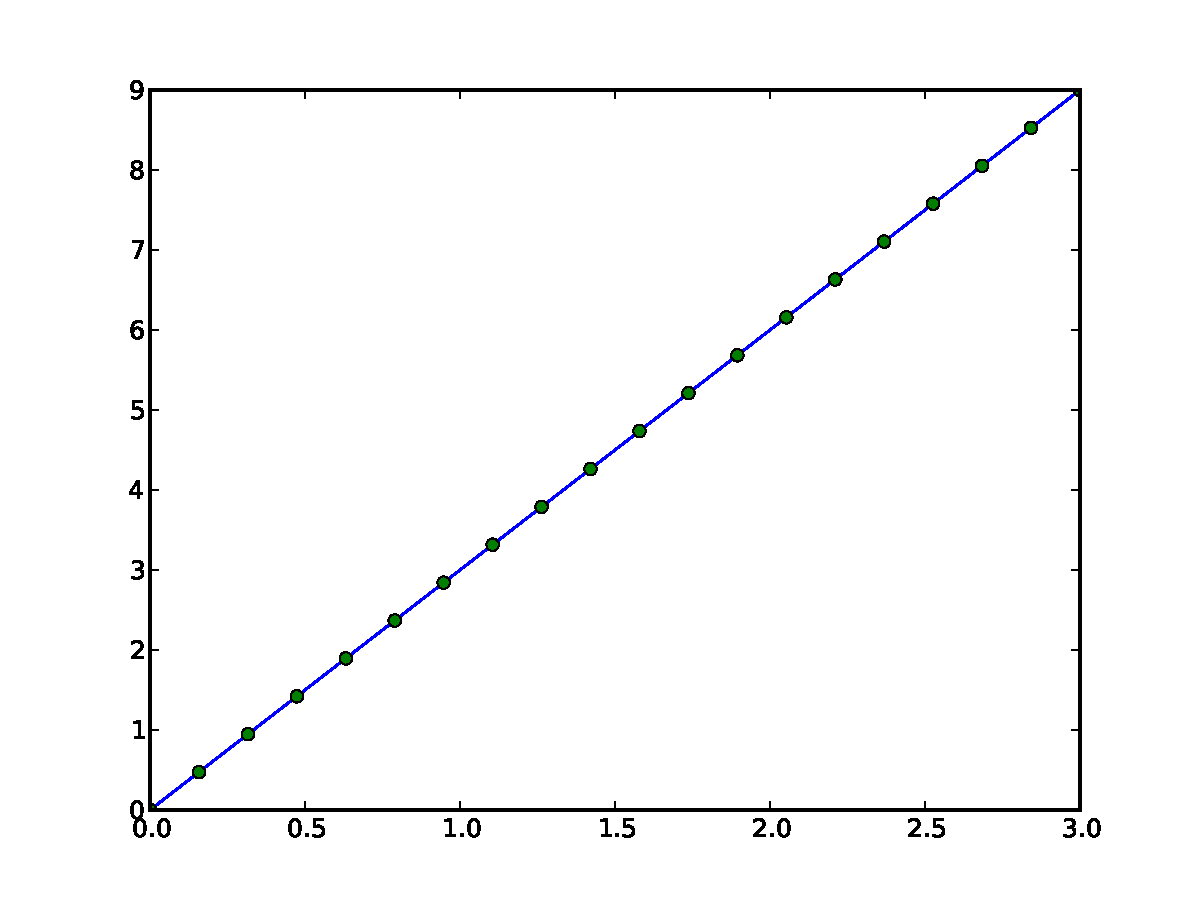
\includegraphics[width=\textwidth]{plwfigis/CursP_2_figure2}

%-------------------------------END CODE
\end{block}
\end{columns}
\end{frame}



%----------------------------FRAME 2 cols------------------------------
\begin{frame}[fragile]\frametitle{Array representation}
\begin{columns}[c]
\column{0.5\textwidth}
\begin{block}{2D arrays (such as images}
%-------------------------------CODE
\tiny
\begin{minted}[bgcolor=mybg,frame=lines,mathescape]{python}
>>> import numpy as np
>>> import matplotlib.pyplot as plt
>>> image = np.random.rand(30, 30)
>>> plt.imshow(image, cmap=plt.cm.hot)    
<matplotlib.image.AxesImage object at 0x25f7950>
>>> plt.colorbar()    
<matplotlib.colorbar.Colorbar instance at 0x2260518>
\end{minted}

%-------------------------------END CODE
\end{block}

\column{0.5\textwidth}
%-------------------------------CODE

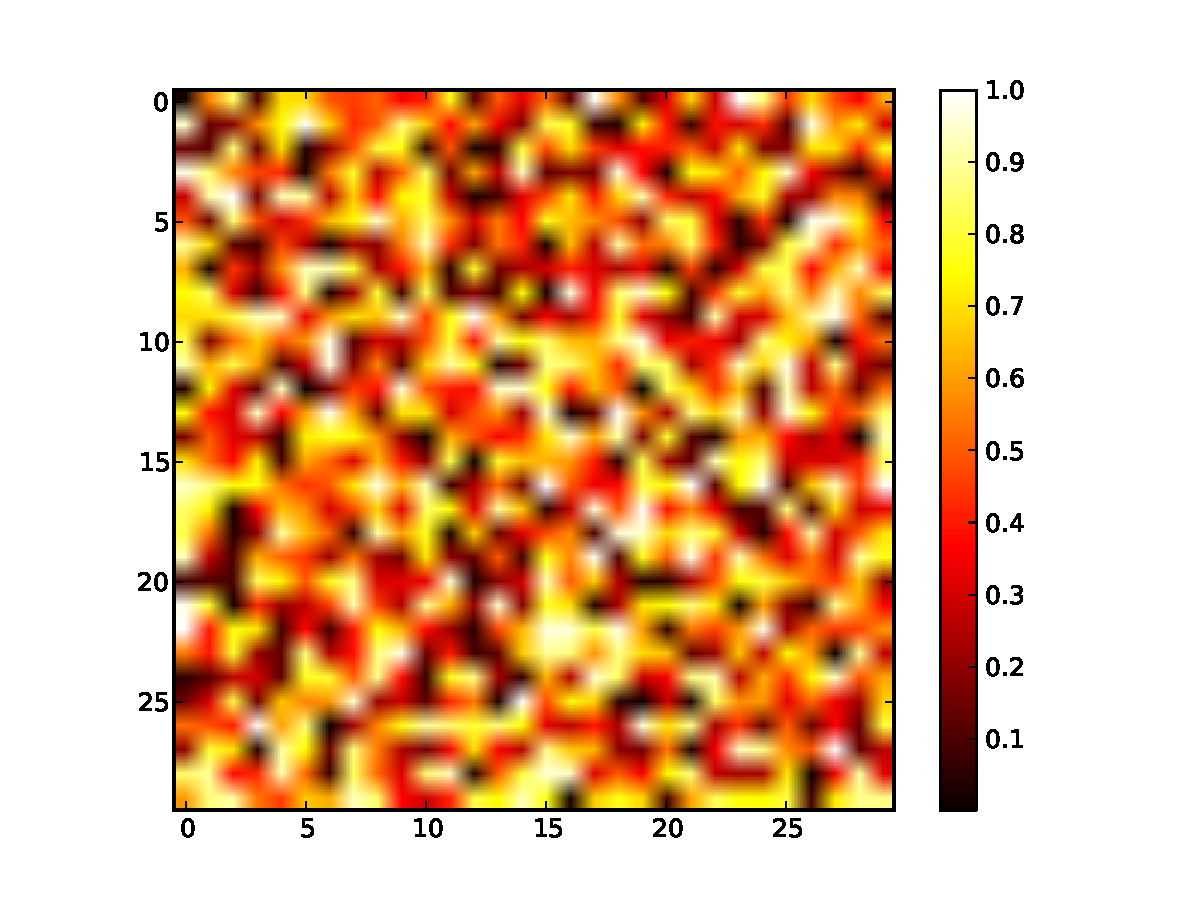
\includegraphics[width=\textwidth]{plwfigis/CursP_2_figure4}

%-------------------------------END CODE
     
\end{columns}
\end{frame}


%----------------------------FRAME 2 cols------------------------------
\begin{frame}[fragile]\frametitle{Array representation}
\begin{block}{3D plotting}
\tiny
\begin{minted} [bgcolor=mybg,frame=lines,bgcolor=mybg,frame=lines,bgcolor=mybg,frame=lines,mathescape]{python}
In [58]: from mayavi import mlab
In [61]: mlab.surf(image)
Out[61]: <enthought.mayavi.modules.surface.Surface object at ...>
In [62]: mlab.axes()
Out[62]: <enthought.mayavi.modules.axes.Axes object at ...>
\end{minted}


\end{block}
\begin{center}
    
    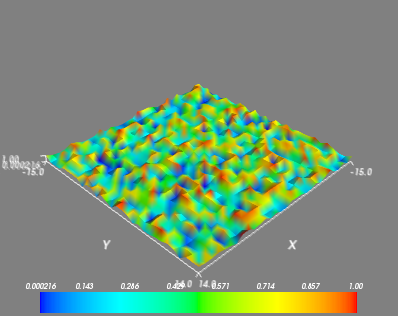
\includegraphics[scale=0.3]{figs/surf1}
\end{center}
\end{frame}

%----------------------------FRAME------------------------------------
\begin{frame}[fragile]\frametitle{Challenge}
\begin{block}{5 minutes challenge}
Plot a sine 1D signal with frequency $10\frac{\text{rad}}{\text{s}}$ sampled everu $0.01$s during $10$s.



\tiny HINT:Use np.sin 
\end{block}
\begin{block}{1 minute challenge}
Plot the previous signal subsampled, one sample every $0.5$s 
\end{block}
\end{frame}

%----------------------------FRAME------------------------------------
\begin{frame}[fragile]\frametitle{Indexing and slicing}
\begin{block}{Indexing}

The items of an array can be accessed and assigned to the same way as other Python sequences (e.g. lists)
\tiny
\begin{minted} [bgcolor=mybg,frame=lines,bgcolor=mybg,frame=lines,bgcolor=mybg,frame=lines,mathescape]{python}
>>> a = np.arange(10)
>>> a
array([0, 1, 2, 3, 4, 5, 6, 7, 8, 9])
>>> a[0], a[2], a[-1]
(0, 2, 9)
\end{minted}
\normalsize
For multidimensional arrays, indexes are tuples of integers:
\tiny
\begin{minted} [bgcolor=mybg,frame=lines,bgcolor=mybg,frame=lines,bgcolor=mybg,frame=lines,mathescape]{python}
>>> a = np.diag(np.arange(3))
>>> a
array([[0, 0, 0],
       [0, 1, 0],
       [0, 0, 2]])
>>> a[1, 1]
1
>>> a[2, 1] = 10 # third line, second column
>>> a
array([[ 0,  0,  0],
       [ 0,  1,  0],
       [ 0, 10,  2]])
>>> a[1]
array([0, 1, 0])
\end{minted}


\end{block}

\end{frame}

%----------------------------FRAME------------------------------------
\begin{frame}[fragile]\frametitle{Indexing and slicing}
\begin{block}{Slicing}
Slicing Arrays, like other Python sequences can also be sliced:
\tiny
\begin{minted} [bgcolor=mybg,frame=lines,bgcolor=mybg,frame=lines,bgcolor=mybg,frame=lines,mathescape]{python}
>>> a = np.arange(10)
>>> a
array([0, 1, 2, 3, 4, 5, 6, 7, 8, 9])
>>> a[2:9:3] # [start:end:step]
array([2, 5, 8])
\end{minted}
\normalsize
Note that the last index is not included!
\tiny
\begin{minted} [bgcolor=mybg,frame=lines,bgcolor=mybg,frame=lines,bgcolor=mybg,frame=lines,mathescape]{python}
>>> a[:4]
array([0, 1, 2, 3])
\end{minted}
\normalsize
All three slice components are not required: by default, start is 0, end is the last and step is 1:
\tiny
\begin{minted} [bgcolor=mybg,frame=lines,bgcolor=mybg,frame=lines,bgcolor=mybg,frame=lines,mathescape]{python}
>>> a[1:3]
array([1, 2])
>>> a[::2]
array([0, 2, 4, 6, 8])
>>> a[3:]
array([3, 4, 5, 6, 7, 8, 9])
\end{minted}


\end{block}

\end{frame}

%----------------------------FRAME 2 cols------------------------------
{
\usebackgroundtemplate{
  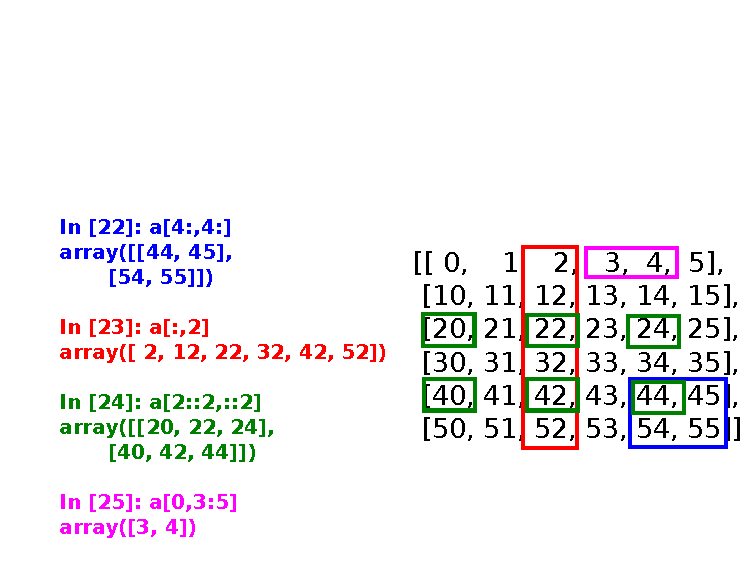
\includegraphics[width=\paperwidth,height=\paperheight]{figs/slicing.pdf}
}

\begin{frame}[fragile]\frametitle{Indexing and slicing}
\vspace{-4cm}
\begin{block}{Small summary}
\tiny
\begin{minted} [bgcolor=mybg,frame=lines,bgcolor=mybg,frame=lines,bgcolor=mybg,frame=lines,mathescape]{python}
a=np.array([np.arange(6)+10*i for i in numpy.arange(6)])
\end{minted}
\end{block}

\end{frame}
}

%----------------------------FRAME------------------------------------
\begin{frame}[fragile]\frametitle{Copies and views}
A slicing operation creates a view on the original array, which is just a way of accessing array data. Thus the original array is not copied in memory.

\begin{block}{1 minute challenge}
Check mutability when accessing an array from a sliced view

\end{block}

\begin{block}{Use .copy() to copy a NumPy array}
\tiny
\begin{minted} [bgcolor=mybg,frame=lines,bgcolor=mybg,frame=lines,bgcolor=mybg,frame=lines,mathescape]{python}
>>> a = np.arange(10)
>>> b = a[::2].copy()  # force a copy
>>> b[0] = 12
>>> a
array([0, 1, 2, 3, 4, 5, 6, 7, 8, 9])
\end{minted}

\end{block}
\end{frame}

%----------------------------FRAME------------------------------------
\begin{frame}[fragile]\frametitle{Copies and views}
\begin{block}{Warning}
This behavior can be surprising at first sight... but it allows to save both memory and time.

As a result, a matrix cannot be made symmetric in-place:
\tiny
\begin{minted} [bgcolor=mybg,frame=lines,bgcolor=mybg,frame=lines,bgcolor=mybg,frame=lines,mathescape]{python}
>>> a = np.ones((100, 100))
>>> a += a.T
>>> a
array([[ 2.,  2.,  2., ...,  2.,  2.,  2.],
       [ 2.,  2.,  2., ...,  2.,  2.,  2.],
       [ 2.,  2.,  2., ...,  2.,  2.,  2.],
       ...,
       [ 3.,  3.,  3., ...,  2.,  2.,  2.],
       [ 3.,  3.,  3., ...,  2.,  2.,  2.],
       [ 3.,  3.,  3., ...,  2.,  2.,  2.]])
\end{minted}
\end{block}
\end{frame}

%----------------------------FRAME------------------------------------
\begin{frame}[fragile]\frametitle{Challenge}
\begin{block}{5 minutes challenge}
Construct an array containing the prime numbers between 1 and 100
\end{block}

\end{frame}

%----------------------------FRAME------------------------------------
\begin{frame}[fragile]\frametitle{Masks}
\begin{block}{Using boolean masks}

\tiny
\begin{minted} [bgcolor=mybg,frame=lines,bgcolor=mybg,frame=lines,bgcolor=mybg,frame=lines,mathescape]{python}


>>> np.random.seed(3)
>>> a = np.random.random_integers(0, 20, 15)
>>> a
array([10,  3,  8,  0, 19, 10, 11,  9, 10,  6,  0, 20, 12,  7, 14])
>>> (a % 3 == 0)
array([False,  True, False,  True, False, False, False,  True, False,
        True,  True, False,  True, False, False], dtype=bool)
>>> mask = (a % 3 == 0)
>>> extract_from_a = a[mask] # or,  a[a%3==0]
>>> extract_from_a           # extract a sub-array with the mask
array([ 3,  0,  9,  6,  0, 12])
\end{minted}
\normalsize
Indexing with a mask can be very useful to assign a new value to a sub-array:
\tiny
\begin{minted} [bgcolor=mybg,frame=lines,bgcolor=mybg,frame=lines,bgcolor=mybg,frame=lines,mathescape]{python}
>>> a[a % 3 == 0] = -1
>>> a
array([10, -1,  8, -1, 19, 10, 11, -1, 10, -1, -1, 20, -1,  7, 14])
\end{minted}
\end{block}
\end{frame}

%----------------------------FRAME------------------------------------
\begin{frame}[fragile]\frametitle{Indexing... more}
\begin{block}{Indexing with an array of int}
\tiny
\begin{minted} [bgcolor=mybg,frame=lines,bgcolor=mybg,frame=lines,bgcolor=mybg,frame=lines,mathescape]{python}
>>> a = np.arange(10)
>>> a
array([0, 1, 2, 3, 4, 5, 6, 7, 8, 9])
\end{minted}
Indexing can be done with an array of integers, where the same index is repeated several time:
\tiny
\begin{minted} [bgcolor=mybg,frame=lines,bgcolor=mybg,frame=lines,bgcolor=mybg,frame=lines,mathescape]{python}
>>> a[[2, 3, 2, 4, 2]]  # note: [2, 3, 2, 4, 2] is a Python list
array([2, 3, 2, 4, 2])
\end{minted}
New values can be assigned with this kind of indexing:
\tiny
\begin{minted} [bgcolor=mybg,frame=lines,bgcolor=mybg,frame=lines,bgcolor=mybg,frame=lines,mathescape]{python}
>>> a[[9, 7]] = -10
>>> a
array([  0,   1,   2,   3,   4,   5,   6, -10,   8, -10])
\end{minted}
When a new array is created by indexing with an array of integers, the new array has the same shape than the array of integers:
\tiny
\begin{minted} [bgcolor=mybg,frame=lines,bgcolor=mybg,frame=lines,bgcolor=mybg,frame=lines,mathescape]{python}
>>> a = np.arange(10)
>>> idx = np.array([[3, 4], [9, 7]])
>>> a[idx]
array([[3, 4],
       [9, 7]])
>>> b = np.arange(10)
\end{minted}
\end{block}
\end{frame}

%----------------------------FRAME------------------------------------
\begin{frame}[fragile]\frametitle{Challenge}
\begin{block}{1 minute challenge}
Check whenever the indexing with int is a view or a copy of the original array
\end{block}

\end{frame}

%----------------------------FRAME 2 cols------------------------------
{
\usebackgroundtemplate{
  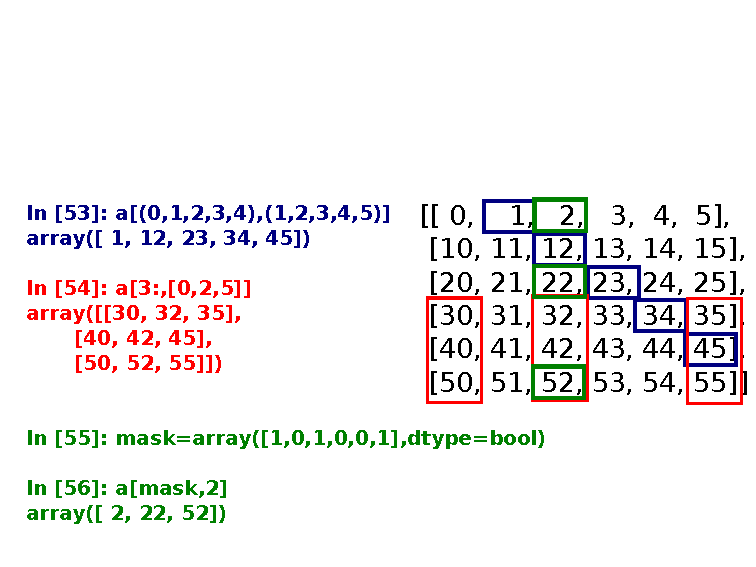
\includegraphics[width=\paperwidth,height=\paperheight]{figs/slicing_int.pdf}
}

\begin{frame}[fragile]\frametitle{Fancy Indexing }
\vspace{-4cm}
\begin{block}{Small summary}
\tiny
\begin{minted} [bgcolor=mybg,frame=lines,bgcolor=mybg,frame=lines,bgcolor=mybg,frame=lines,mathescape]{python}
a=np.array([np.arange(6)+10*i for i in numpy.arange(6)])
\end{minted}
\end{block}

\end{frame}
}

%----------------------------FRAME------------------------------------
\begin{frame}[fragile]\frametitle{Indexing}

\begin{block}{Adding axes while indexing}



Indexing with the np.newaxis object allows us to add an axis to an array:
\tiny
\begin{minted} [bgcolor=mybg,frame=lines,bgcolor=mybg,frame=lines,bgcolor=mybg,frame=lines,mathescape]{python}


>>> z = np.array([1, 2, 3])
>>> z
array([1, 2, 3])
>>> z[:, np.newaxis]
array([[1],
       [2],
       [3]])
>>> z[np.newaxis, :]
array([[1, 2, 3]])

\end{minted}
\end{block}
\end{frame}


\subsection{Operating with Arrays}
%----------------------------FRAME------------------------------------
\begin{frame}[fragile]\frametitle{Numerical Operations}
\begin{block}{Elementwise operations}
With scalars:
\tiny
\begin{minted} [bgcolor=mybg,frame=lines,bgcolor=mybg,frame=lines,bgcolor=mybg,frame=lines,mathescape]{python}


>>> a = np.array([1, 2, 3, 4])
>>> a + 1
array([2, 3, 4, 5])
>>> 2**a
array([ 2,  4,  8, 16])
\end{minted}
\normalsize
All arithmetic operates elementwise:
\tiny
\begin{minted} [bgcolor=mybg,frame=lines,bgcolor=mybg,frame=lines,bgcolor=mybg,frame=lines,mathescape]{python}
>>> b = np.ones(4) + 1
>>> a - b
array([-1.,  0.,  1.,  2.])
>>> a * b
array([ 2.,  4.,  6.,  8.])
>>> j = np.arange(5)
>>> 2**(j + 1) - j
array([ 2,  3,  6, 13, 28])
\end{minted}
\end{block}

\end{frame}

%----------------------------FRAME------------------------------------
\begin{frame}[fragile]\frametitle{Numerical Operations}
\begin{block}{Warning}


Array multiplication is not matrix multiplication:
\tiny
\begin{minted} [bgcolor=mybg,frame=lines,bgcolor=mybg,frame=lines,bgcolor=mybg,frame=lines,mathescape]{python}


>>> c = np.ones((3, 3))
>>> c * c                   # NOT matrix multiplication!
array([[ 1.,  1.,  1.],
       [ 1.,  1.,  1.],
       [ 1.,  1.,  1.]])

\end{minted}
\end{block}
\begin{block}{Use .dot()}


Note Matrix multiplication:
\tiny
\begin{minted} [bgcolor=mybg,frame=lines,bgcolor=mybg,frame=lines,bgcolor=mybg,frame=lines,mathescape]{python}


>>> c.dot(c)
array([[ 3.,  3.,  3.],
       [ 3.,  3.,  3.],
       [ 3.,  3.,  3.]])

\end{minted}
\end{block}
\end{frame}

%----------------------------FRAME------------------------------------
\begin{frame}[fragile]\frametitle{Numerical Operations}
\begin{block}{More operations}

\tiny
Comparisons:
\begin{minted} [bgcolor=mybg,frame=lines,bgcolor=mybg,frame=lines,bgcolor=mybg,frame=lines,mathescape]{python}


>>> a = np.array([1, 2, 3, 4])
>>> b = np.array([4, 2, 2, 4])
>>> a == b
array([False,  True, False,  True], dtype=bool)
>>> a > b
array([False, False,  True, False], dtype=bool)
\end{minted}

Logical operations:
\tiny
\begin{minted} [bgcolor=mybg,frame=lines,bgcolor=mybg,frame=lines,bgcolor=mybg,frame=lines,mathescape]{python}


>>> a = np.array([1, 1, 0, 0], dtype=bool)
>>> b = np.array([1, 0, 1, 0], dtype=bool)
>>> np.logical_or(a, b)
array([ True,  True,  True, False], dtype=bool)
>>> np.logical_and(a, b)
array([ True, False, False, False], dtype=bool)
\end{minted}
\end{block}
\end{frame}
%----------------------------FRAME------------------------------------
\begin{frame}[fragile]\frametitle{Numerical Operations}
\begin{block}{More operations}
Shape mismatches:
\tiny
\begin{minted} [bgcolor=mybg,frame=lines,bgcolor=mybg,frame=lines,bgcolor=mybg,frame=lines,mathescape]{python}
>>> a = np.arange(4)
>>> a
array([0, 1, 2, 3])
>>> a + np.array([1, 2])    
Traceback (most recent call last):
File "<stdin>", line 1, in <module>
ValueError: shape mismatch: objects cannot be broadcast to a single shape
\end{minted}
\normalsize
'Broadcast'? We'll return to that later.
\end{block}
\end{frame}

%----------------------------FRAME------------------------------------
\begin{frame}[fragile]\frametitle{Challenge}
\begin{block}{3 minutes challenge}
Generate arrays [2**0, 2**1, 2**2, 2**3, 2**4] 

and $a_j = 2^{3*j} - j$
\end{block}

\end{frame}

%----------------------------FRAME 2 cols------------------------------
\begin{frame}[fragile]\frametitle{Numerical Operations}
\begin{columns}[c]
\column{0.5\textwidth}
\begin{block}{Basic reductions}


Computing sums:
\tiny
\begin{minted} [bgcolor=mybg,frame=lines,bgcolor=mybg,frame=lines,bgcolor=mybg,frame=lines,mathescape]{python}


>>> x = np.array([1, 2, 3, 4])
>>> np.sum(x)
10
>>> x.sum()
10

\end{minted}
\normalsize
Sum by rows and by columns:
\tiny
\begin{minted} [bgcolor=mybg,frame=lines,bgcolor=mybg,frame=lines,bgcolor=mybg,frame=lines,mathescape]{python}
>>> x = np.array([[1, 1], [2, 2]])
>>> x
array([[1, 1],
       [2, 2]])
>>> x.sum(axis=0)   # columns (first dimension)
array([3, 3])
>>> x[:, 0].sum(), x[:, 1].sum()
(3, 3)
>>> x.sum(axis=1)   # rows (second dimension)
array([2, 4])
>>> x[0, :].sum(), x[1, :].sum()
(2, 4)
\end{minted}
\end{block}
\column{0.5\textwidth}
\vspace{-3cm}
  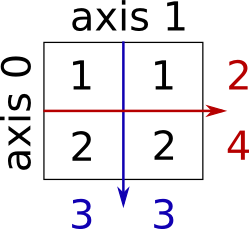
\includegraphics[scale=0.6]{figs/reductions}
\end{columns}
\end{frame}

%----------------------------FRAME 2 cols------------------------------
\begin{frame}[fragile]\frametitle{Numerical Operations}
\begin{columns}[c]
\column{0.5\textwidth}
\begin{block}{Statistics}
\tiny
\begin{minted} [bgcolor=mybg,frame=lines,bgcolor=mybg,frame=lines,bgcolor=mybg,frame=lines,mathescape]{python}

>>> x = np.array([1, 2, 3, 1])
>>> y = np.array([[1, 2, 3], [5, 6, 1]])
>>> x.mean()
1.75
>>> np.median(x)
1.5
>>> np.median(y, axis=-1) # last axis
array([ 2.,  5.])
\end{minted}
\begin{minted} [bgcolor=mybg,frame=lines,bgcolor=mybg,frame=lines,bgcolor=mybg,frame=lines,mathescape]{python}
>>> x.std()  # full population standard dev.
0.82915619758884995
\end{minted}

\end{block}

\begin{block}{Logical operations}
\tiny
\begin{minted} [bgcolor=mybg,frame=lines,bgcolor=mybg,frame=lines,bgcolor=mybg,frame=lines,mathescape]{python}
>>> np.all([True, True, False])
False
>>> np.any([True, True, False])
True
\end{minted}
\end{block}

\column{0.5\textwidth}
\begin{block}{Extrema}
\tiny
\begin{minted} [bgcolor=mybg,frame=lines,bgcolor=mybg,frame=lines,bgcolor=mybg,frame=lines,mathescape]{python}
>>> x = np.array([1, 3, 2])
>>> x.min()
1
>>> x.max()
3
\end{minted}
\begin{minted} [bgcolor=mybg,frame=lines,bgcolor=mybg,frame=lines,bgcolor=mybg,frame=lines,mathescape]{python}
>>> x.argmin()  # index of minimum
0
>>> x.argmax()  # index of maximum
1
\end{minted}
\end{block}



\begin{block}{Note: very usefull}
\tiny
\begin{minted} [bgcolor=mybg,frame=lines,bgcolor=mybg,frame=lines,bgcolor=mybg,frame=lines,mathescape]{python}
>>> a = np.zeros((100, 100))
>>> np.any(a != 0)
False
>>> np.all(a == a)
True
\end{minted}
\end{block}


\end{columns}
\end{frame}


%----------------------------FRAME 2 cols------------------------------
\begin{frame}[fragile]\frametitle{Guided exemple}
\begin{columns}[c]
\column{0.6\textwidth}
\tiny
%-------------------------------CODE
\begin{minted}[bgcolor=mybg,frame=lines,mathescape]{python}
>>> import numpy as np
>>> import matplotlib.pyplot as plt
>>> # We can first plot the data:
>>> data = np.loadtxt('challenges/populations.txt')
>>> year, hares, lynxes, carrots = data.T  # trick: columns to variables
>>> plt.plot(year, hares, year, lynxes, year, carrots)
[<matplotlib.lines.Line2D object at 0x29f6d10>, <matplotlib.lines.Line2D object at 0x29f6e10>, <matplotlib.lines.Line2D object at 0x29fa350>]
>>> plt.legend(('Hare', 'Lynx', 'Carrot'), loc=(1.05, 0.5))
<matplotlib.legend.Legend object at 0x29fac90>
>>> # The mean populations over time:
>>> populations = data[:,1:]
>>> print populations.mean(axis=0)
[ 34080.95238095  20166.66666667  42400.        ]
>>> # [ 34080.95238095,  20166.66666667,  42400.        ]
>>> # The sample standard deviations:
>>> print populations.std(axis=0, ddof=1)
[ 21413.98185877  16655.99991995   3404.55577132]
>>> # [ 21413.98185877,  16655.99991995,   3404.55577132]
>>> # Which species has the highest population each year?
>>> print np.argmax(populations, axis=1)
[2 2 0 0 1 1 2 2 2 2 2 2 0 0 0 1 2 2 2 2 2]
>>> # [2, 2, 0, 0, 1, 1, 2, 2, 2, 2, 2, 2, 0, 0, 0, 1, 2, 2, 2, 2, 2]
\end{minted}

%-------------------------------END CODE
\column{0.4\textwidth}
%-------------------------------CODE
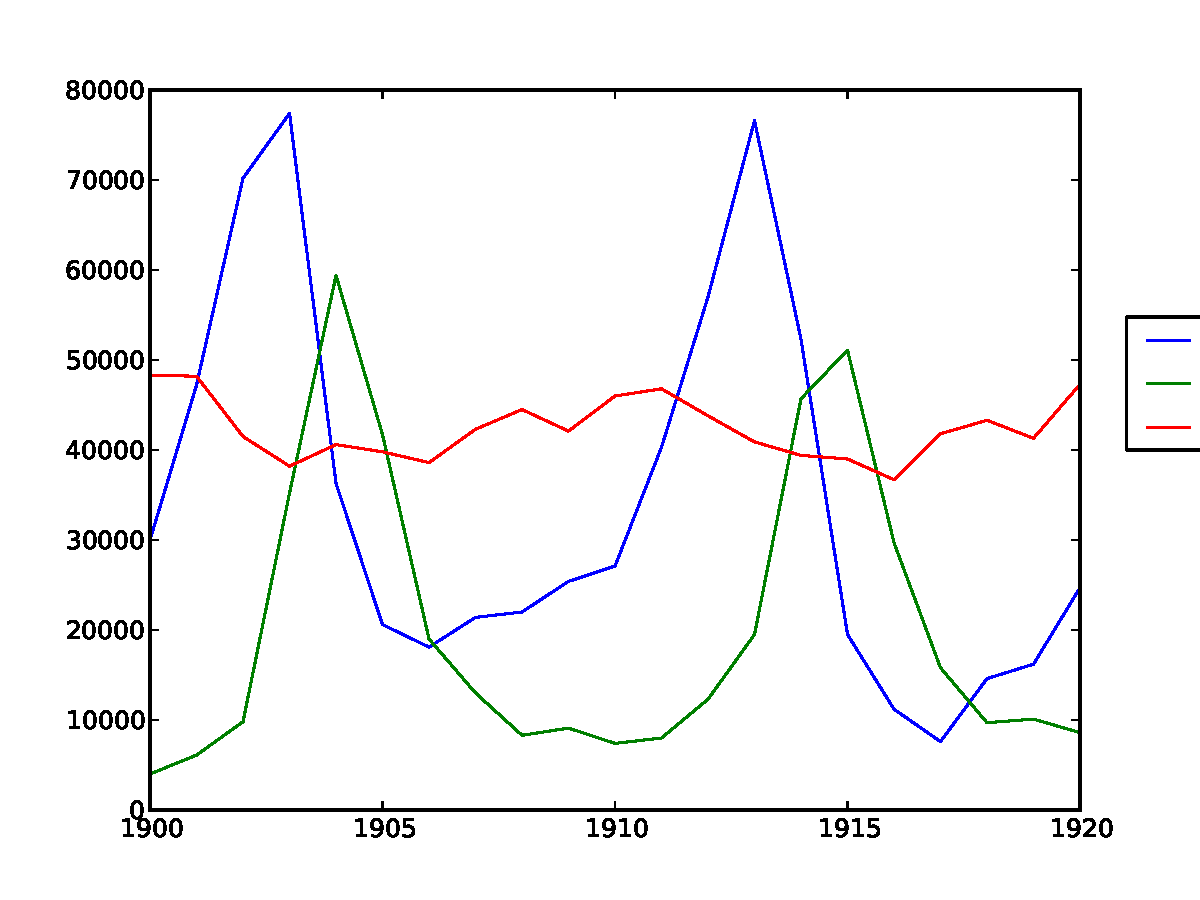
\includegraphics[width=\textwidth]{plwfigis/CursP_2_figure6}

%-------------------------------END CODE
\end{columns}
\end{frame}

%----------------------------FRAME 2 cols------------------------------
\begin{frame}[fragile]\frametitle{Guided exemple}
\tiny
%-------------------------------CODE
\begin{minted}[bgcolor=mybg,frame=lines,mathescape]{python}
>>> import numpy as np
>>> import matplotlib.pyplot as plt
>>> n_stories = 1000 # number of walkers
>>> t_max = 200      # time during which we follow the walker
>>> # We randomly choose all the steps 1 or -1 of the walk
>>> t = np.arange(t_max)
>>> steps = 2 * np.random.random_integers(0, 1, (n_stories, t_max)) - 1
>>> print np.unique(steps) # Verification: all steps are 1 or -1
[-1  1]
>>> # [-1,  1]
>>> # We build the walks by summing steps along the time
>>> positions = np.cumsum(steps, axis=1) # axis = 1: dimension of time
>>> sq_distance = positions**2
>>> # We get the mean in the axis of the stories
>>> mean_sq_distance = np.mean(sq_distance, axis=0)
>>> # Plot the results:
>>> plt.figure(figsize=(4, 3))
<matplotlib.figure.Figure object at 0x24a2a90>
>>> plt.plot(t, np.sqrt(mean_sq_distance), 'g.', t, np.sqrt(t), 'y-')
[<matplotlib.lines.Line2D object at 0x2499650>, <matplotlib.lines.Line2D object at 0x248af90>]
>>> plt.xlabel(r"$t$")
<matplotlib.text.Text object at 0x26017d0>
>>> plt.ylabel(r"$\sqrt{\langle (\delta x)^2 \rangle}$")
<matplotlib.text.Text object at 0x279cf90>
\end{minted}

%-------------------------------END CODE
\end{frame}

%----------------------------FRAME 2 cols------------------------------
\begin{frame}[fragile]\frametitle{}
\begin{columns}[c]
\column{0.7\textwidth}

%-------------------------------CODE
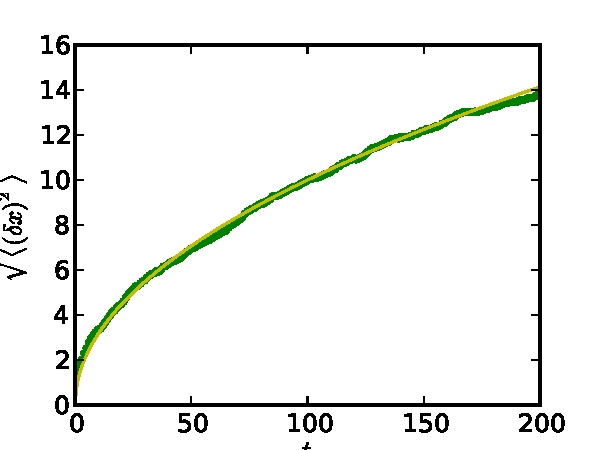
\includegraphics[width=\textwidth]{plwfigis/CursP_2_figure8}

%-------------------------------END CODE
\column{0.3\textwidth}

\end{columns}
\end{frame}


%----------------------------FRAME------------------------------------
\begin{frame}[fragile]\frametitle{Numerical Operations}
\begin{block}{Broadcasting}
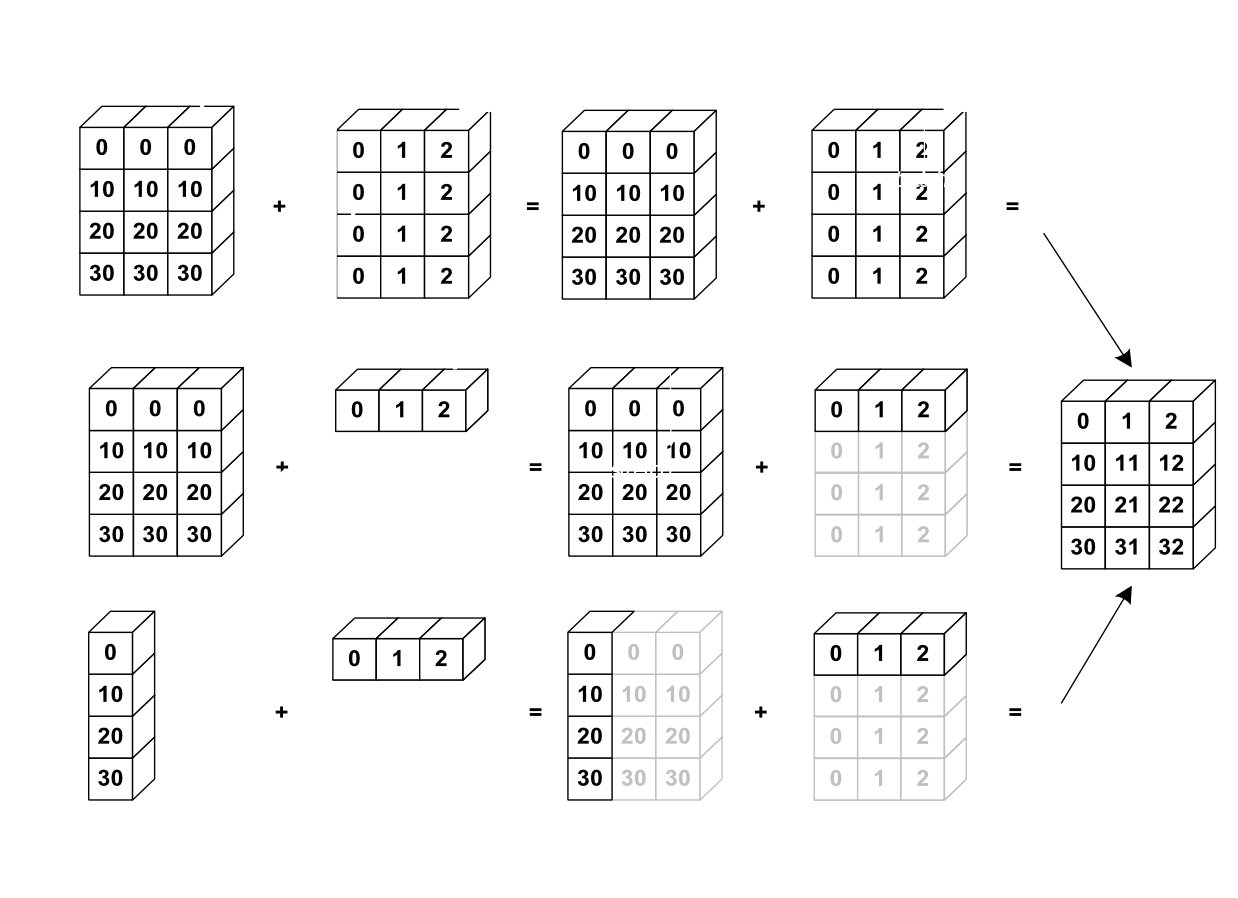
\includegraphics[scale=0.25]{figs/numpy_broadcasting}

\end{block}

\end{frame}

%----------------------------FRAME------------------------------------
\begin{frame}[fragile]\frametitle{Challenge}
\begin{block}{1 minute challenge}
Verify that broadcasting works as specified
\end{block}

\end{frame}

%----------------------------FRAME------------------------------------
\begin{frame}[fragile]\frametitle{Numerical Operations}
\begin{block}{Broadcasting example}
Let’s construct an array of distances (in miles) between cities of Europe.
\tiny
%-------------------------------CODE
\begin{minted}[bgcolor=mybg,frame=lines,mathescape]{python}
>>> mileposts = np.array([0, 198, 303, 736, 871, 1175, 1475, 1544,1913, 2448])
>>> distance_array = np.abs(mileposts - mileposts[:, np.newaxis])
>>> distance_array
array([[   0,  198,  303,  736,  871, 1175, 1475, 1544, 1913, 2448],
       [ 198,    0,  105,  538,  673,  977, 1277, 1346, 1715, 2250],
       [ 303,  105,    0,  433,  568,  872, 1172, 1241, 1610, 2145],
       [ 736,  538,  433,    0,  135,  439,  739,  808, 1177, 1712],
       [ 871,  673,  568,  135,    0,  304,  604,  673, 1042, 1577],
       [1175,  977,  872,  439,  304,    0,  300,  369,  738, 1273],
       [1475, 1277, 1172,  739,  604,  300,    0,   69,  438,  973],
       [1544, 1346, 1241,  808,  673,  369,   69,    0,  369,  904],
       [1913, 1715, 1610, 1177, 1042,  738,  438,  369,    0,  535],
       [2448, 2250, 2145, 1712, 1577, 1273,  973,  904,  535,    0]])
\end{minted}

%-------------------------------END CODE

\end{block}

\end{frame}

%----------------------------FRAME------------------------------------
\begin{frame}[fragile]\frametitle{Numerical Operations}
\begin{block}{Array shape manipulation}
\tiny
Flattening
\begin{minted} [bgcolor=mybg,frame=lines,bgcolor=mybg,frame=lines,bgcolor=mybg,frame=lines,mathescape]{python}
>>> a = np.array([[1, 2, 3], [4, 5, 6]])
>>> a.ravel()
array([1, 2, 3, 4, 5, 6])
>>> a.T
array([[1, 4],
       [2, 5],
       [3, 6]])
>>> a.T.ravel()
array([1, 4, 2, 5, 3, 6])
\end{minted}

Reshaping
\begin{minted} [bgcolor=mybg,frame=lines,bgcolor=mybg,frame=lines,bgcolor=mybg,frame=lines,mathescape]{python}
>>> a.shape
(2, 3)
>>> b = a.ravel()
>>> b.reshape((2, 3))
array([[1, 2, 3],
       [4, 5, 6]])
\end{minted}


\end{block}

\end{frame}

%----------------------------FRAME------------------------------------
\begin{frame}[fragile]\frametitle{Example of use for Phisicists}
\begin{block}{Block matrices and vectors (and tensors)}
Vector space: quantum level $\otimes$ spin
\[
\check{\psi}=\left(\begin{matrix}\hat{\psi}_1 \\ \hat{\psi}_2\end{matrix}\right),\,\,\,\hat{\psi}_1=\left(\begin{matrix}\psi_{1\uparrow} \\ \psi_{1\downarrow}\end{matrix}\right),\,\,\,\hat{\psi}_2=\left(\begin{matrix}\psi_{2\uparrow} \\ \psi_{2\downarrow}\end{matrix}\right)
\]
In short: for block matrices and vectors, it can be useful to preserve the block structure.
\tiny
\begin{minted} [bgcolor=mybg,frame=lines,bgcolor=mybg,frame=lines,bgcolor=mybg,frame=lines,mathescape]{python}
>>> psi = np.zeros((2, 2))   # dimensions: level, spin
>>> psi[0, 1] # <-- psi_{1,downarrow}
0.0
\end{minted}

\end{block}

\end{frame}

%----------------------------FRAME------------------------------------
\begin{frame}[fragile]\frametitle{Example of use for Phisicists}
\begin{block}{Block matrices and vectors (and tensors)}
Linear operators on such block vectors have similar block structure:
\small
\[
\check{H}=\left(\begin{matrix}\hat{h}_{11} & \hat{V} \\ \hat{V}^\dagger & \hat{h}_{22} \end{matrix}\right),\,\,\check{h}_{11}=\left(\begin{matrix}\epsilon_{1\uparrow} & 0 \\ 0 & \epsilon_{1\downarrow} \end{matrix}\right)
\]
\tiny
\begin{minted} [bgcolor=mybg,frame=lines,bgcolor=mybg,frame=lines,bgcolor=mybg,frame=lines,mathescape]{python}
>>> H = np.zeros((2, 2, 2, 2)) # dimensions: level1, level2, spin1, spin2
>>> h_11 = H[0,0,:,:]
>>> V = H[0,1]
\end{minted}
\normalsize
Doing the matrix product: get rid of the block structure, do the 4x4 matrix product, then put it back
\small
\[
\check{H}\check{\psi}
\]
\tiny
\begin{minted} [bgcolor=mybg,frame=lines,bgcolor=mybg,frame=lines,bgcolor=mybg,frame=lines,mathescape]{python}
>>> def mdot(operator, psi):
...     return operator.transpose(0, 2, 1, 3).reshape(4, 4).dot(
...                psi.reshape(4)).reshape(2, 2)
\end{minted}

\end{block}

\end{frame}

%----------------------------FRAME------------------------------------
\begin{frame}[fragile]\frametitle{Numerical Operations}
\begin{block}{Sorting data}
Sorting along an axis:
\tiny
\begin{minted} [bgcolor=mybg,frame=lines,bgcolor=mybg,frame=lines,bgcolor=mybg,frame=lines,mathescape]{python}
>>> a = np.array([[4, 3, 5], [1, 2, 1]])
>>> b = np.sort(a, axis=1)
>>> b
array([[3, 4, 5],
       [1, 1, 2]])
\end{minted}

\normalsize
In-place sort:
\tiny
\begin{minted} [bgcolor=mybg,frame=lines,bgcolor=mybg,frame=lines,bgcolor=mybg,frame=lines,mathescape]{python}
>>> a.sort(axis=1)
>>> a
array([[3, 4, 5],
       [1, 1, 2]])
\end{minted}
\end{block}

\end{frame}

%----------------------------FRAME------------------------------------
\begin{frame}[fragile]\frametitle{Numerical Operations}
\begin{block}{Getting indices of the sort}
\tiny
\begin{minted} [bgcolor=mybg,frame=lines,bgcolor=mybg,frame=lines,bgcolor=mybg,frame=lines,mathescape]{python}
>>> a = np.array([4, 3, 1, 2])
>>> j = np.argsort(a)
>>> j
array([2, 3, 1, 0])
>>> a[j]
array([1, 2, 3, 4])
\end{minted}
\end{block}
\begin{block}{Also getting indices of min and max}
\tiny
\begin{minted} [bgcolor=mybg,frame=lines,bgcolor=mybg,frame=lines,bgcolor=mybg,frame=lines,mathescape]{python}
>>> a = np.array([4, 3, 1, 2])
>>> j_max = np.argmax(a)
>>> j_min = np.argmin(a)
>>> j_max, j_min
(0, 2)
\end{minted}



\end{block}

\end{frame}

%----------------------------FRAME------------------------------------
\begin{frame}[fragile]\frametitle{Challenge}
\begin{block}{5 minutes multy-challenge}
\begin{enumerate}
    \item Form the 2-D array (without typing it in explicitly):
\tiny
\begin{minted} [bgcolor=mybg,frame=lines,bgcolor=mybg,frame=lines,bgcolor=mybg,frame=lines,mathescape]{python}
1  6 11
2  7 12
3  8 13
4  9 14
5 10 15
\end{minted}
\normalsize
and generate a new array containing its 2nd and 4th rows.
\item Divide each column of the array:
\tiny
\begin{minted} [bgcolor=mybg,frame=lines,bgcolor=mybg,frame=lines,bgcolor=mybg,frame=lines,mathescape]{python}
>>> a = np.arange(25).reshape(5, 5)
\end{minted}

\normalsize
elementwise with the array b = np.array([1., 5, 10, 15, 20]). (Hint: np.newaxis).

\end{enumerate}

\end{block}

\end{frame}
%----------------------------FRAME------------------------------------
\begin{frame}[fragile]\frametitle{Challenge}
\begin{block}{Worked challenge}
From Lena picture get these modifications

\centering
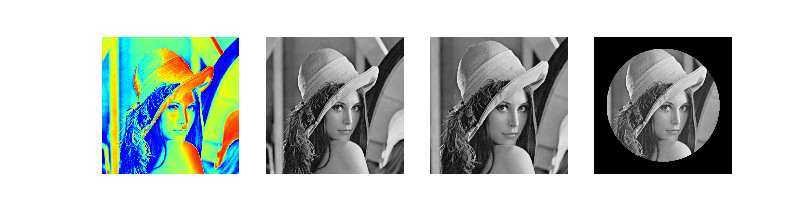
\includegraphics[scale=0.5]{figs/lenas}
\end{block}
\begin{block}{Lena picture}
\tiny
\begin{minted} [bgcolor=mybg,frame=lines,bgcolor=mybg,frame=lines,bgcolor=mybg,frame=lines,mathescape]{python}
>>> from scipy import misc
>>> lena = misc.lena()
\end{minted}

\end{block}




\end{frame}


%----------------------------FRAME------------------------------------
\begin{frame}[fragile]\frametitle{Solution to Lena}
\begin{block}{First image}
\begin{minted} [bgcolor=mybg,frame=lines,bgcolor=mybg,frame=lines,bgcolor=mybg,frame=lines,mathescape]{python}
In [3]: import pylab as plt
In [4]: lena = misc.lena()
In [5]: plt.imshow(lena)
\end{minted}

\end{block}
\pause
\begin{block}{Second image}
\begin{minted} [bgcolor=mybg,frame=lines,bgcolor=mybg,frame=lines,bgcolor=mybg,frame=lines,mathescape]{python}
In [6]: plt.imshow(lena, cmap=plt.cm.gray)
\end{minted}

\end{block}
\pause
\begin{block}{Third image}
\begin{minted} [bgcolor=mybg,frame=lines,bgcolor=mybg,frame=lines,bgcolor=mybg,frame=lines,mathescape]{python}
In [9]: crop_lena = lena[30:-30,30:-30]
\end{minted}

\end{block}


\end{frame}
%----------------------------FRAME------------------------------------
\begin{frame}[fragile]\frametitle{Solution to Lena}


\begin{block}{Last image}
\tiny
\begin{minted} [bgcolor=mybg,frame=lines,bgcolor=mybg,frame=lines,bgcolor=mybg,frame=lines,mathescape]{python}
In [15]: y, x = np.ogrid[0:512,0:512] # x and y indices of pixels
In [16]: y.shape, x.shape
Out[16]: ((512, 1), (1, 512))
In [17]: centerx, centery = (256, 256) # center of the image
In [18]: mask = ((y - centery)**2 + (x - centerx)**2) > 230**2 # circle
In [19]: lena[mask] = 0
In [20]: plt.imshow(lena)
\end{minted}

\end{block}

\end{frame}



\subsection{Advanced Arrays (ndarrays)}
%----------------------------FRAME------------------------------------
\begin{frame}[fragile]\frametitle{More elaborated arrays}
\begin{block}{Casting}
“Bigger” type wins in mixed-type operations:
\tiny
\begin{minted} [bgcolor=mybg,frame=lines,bgcolor=mybg,frame=lines,bgcolor=mybg,frame=lines,mathescape]{python}
>>> np.array([1, 2, 3]) + 1.5
array([ 2.5,  3.5,  4.5])
\end{minted}

\end{block}
\begin{block}{Assignment never changes the type!}
\tiny
\begin{minted} [bgcolor=mybg,frame=lines,bgcolor=mybg,frame=lines,bgcolor=mybg,frame=lines,mathescape]{python}
>>> a = np.array([1, 2, 3])
>>> a.dtype
dtype('int64')
>>> a[0] = 1.9     # <-- float is truncated to integer
>>> a
array([1, 2, 3])
\end{minted}

\end{block}

\end{frame}

%----------------------------FRAME------------------------------------
\begin{frame}[fragile]\frametitle{More elaborated arrays}
\begin{block}{Forced casts:}
\tiny
\begin{minted} [bgcolor=mybg,frame=lines,bgcolor=mybg,frame=lines,bgcolor=mybg,frame=lines,mathescape]{python}
>>> a = np.array([1.7, 1.2, 1.6])
>>> b = a.astype(int)  # <-- truncates to integer
>>> b
array([1, 1, 1])
\end{minted}

\end{block}
\begin{block}{Rounding:}


\tiny
\begin{minted} [bgcolor=mybg,frame=lines,bgcolor=mybg,frame=lines,bgcolor=mybg,frame=lines,mathescape]{python}
>>> a = np.array([1.2, 1.5, 1.6, 2.5, 3.5, 4.5])
>>> b = np.around(a)
>>> b                    # still floating-point
array([ 1., 2., 2., 2., 4., 4.])
>>> c = np.around(a).astype(int)
>>> c
array([ 1, 2, 2, 2, 4, 4])
\end{minted}

\end{block}

\end{frame}

%----------------------------FRAME------------------------------------
\begin{frame}[fragile]\frametitle{ Structured data types}
\begin{block}{Sensor example}
\begin{itemize}
    \item sensor code (4 character string)	 
\item position (float)	 
\item value (float)
\end{itemize}
\tiny
\begin{minted} [bgcolor=mybg,frame=lines,bgcolor=mybg,frame=lines,bgcolor=mybg,frame=lines,mathescape]{python}
>>> samples = np.zeros((6,), dtype=[('sensor_code', 'S4'),
...                                 ('position', float), ('value', float)])
>>> samples.ndim
1
>>> samples.shape
(6,)
>>> samples.dtype.names
('sensor_code', 'position', 'value')
\end{minted}

\end{block}

\end{frame}
%----------------------------FRAME------------------------------------
\begin{frame}[fragile]\frametitle{Structured data types}
\begin{block}{Assignment}
\tiny
\begin{minted} [bgcolor=mybg,frame=lines,bgcolor=mybg,frame=lines,bgcolor=mybg,frame=lines,mathescape]{python}
>>> samples[:] = [('ALFA',   1, 0.37), ('BETA', 1, 0.11), ('TAU', 1,   0.13),
...               ('ALFA', 1.5, 0.37), ('ALFA', 3, 0.11), ('TAU', 1.2, 0.13)]
>>> samples
array([('ALFA', 1.0, 0.37), ('BETA', 1.0, 0.11), ('TAU', 1.0, 0.13),
       ('ALFA', 1.5, 0.37), ('ALFA', 3.0, 0.11), ('TAU', 1.2, 0.13)],
      dtype=[('sensor_code', '|S4'), ('position', '<f8'), ('value', '<f8')])
\end{minted}
\end{block}
\begin{block}{Field access works by indexing with field names:}
\tiny
\begin{minted} [bgcolor=mybg,frame=lines,bgcolor=mybg,frame=lines,bgcolor=mybg,frame=lines,mathescape]{python}
>>> samples['sensor_code']
array(['ALFA', 'BETA', 'TAU', 'ALFA', 'ALFA', 'TAU'],
      dtype='|S4')
>>> samples['value']
array([ 0.37,  0.11,  0.13,  0.37,  0.11,  0.13])
>>> samples[0]
('ALFA', 1.0, 0.37)

>>> samples[0]['sensor_code'] = 'TAU'
>>> samples[0]
('TAU', 1.0, 0.37)
\end{minted}

\end{block}

\end{frame}

%----------------------------FRAME------------------------------------
\begin{frame}[fragile]\frametitle{Structured Data Types}
\begin{block}{Multiple fields at once:}
\tiny
\begin{minted} [bgcolor=mybg,frame=lines,bgcolor=mybg,frame=lines,bgcolor=mybg,frame=lines,mathescape]{python}
>>> samples[['position', 'value']]
array([(1.0, 0.37), (1.0, 0.11), (1.0, 0.13), (1.5, 0.37), (3.0, 0.11),
       (1.2, 0.13)],
      dtype=[('position', '<f8'), ('value', '<f8')])
\end{minted}

\end{block}
\begin{block}{Fancy indexing works, as usual:}
\tiny
\begin{minted} [bgcolor=mybg,frame=lines,bgcolor=mybg,frame=lines,bgcolor=mybg,frame=lines,mathescape]{python}
>>> samples[samples['sensor_code'] == 'ALFA']
array([('ALFA', 1.5, 0.37), ('ALFA', 3.0, 0.11)],
      dtype=[('sensor_code', '|S4'), ('position', '<f8'), ('value', '<f8')])
\end{minted}

\end{block}


\end{frame}

%----------------------------FRAME------------------------------------
\begin{frame}[fragile]\frametitle{Under the Hood}
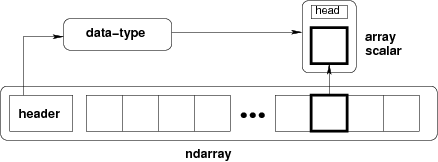
\includegraphics[scale=0.6]{figs/ndarray}
\end{frame}
\subsection{Advanced Operations}
%----------------------------FRAME------------------------------------
\begin{frame}[fragile]\frametitle{Advanced Operations}
\begin{block}{Polinomials}
Numpy also contains polynomials in different bases, for instance $3x^2+2x-1$
\tiny
\begin{minted} [bgcolor=mybg,frame=lines,bgcolor=mybg,frame=lines,bgcolor=mybg,frame=lines,mathescape]{python}
>>> p = np.poly1d([3, 2, -1])
>>> p(0)
-1
>>> p.roots
array([-1.        ,  0.33333333])
>>> p.order
2
\end{minted}

\end{block}
\begin{block}{Fitting...}
\tiny
\begin{minted} [bgcolor=mybg,frame=lines,bgcolor=mybg,frame=lines,bgcolor=mybg,frame=lines,mathescape]{python}
>>> x = np.linspace(0, 1, 20)
>>> y = np.cos(x) + 0.3*np.random.rand(20)
>>> p = np.poly1d(np.polyfit(x, y, 3))
\end{minted}

\end{block}

\end{frame}

%----------------------------FRAME 2 cols------------------------------
\begin{frame}[fragile]\frametitle{Advanced Operations}
\begin{columns}[c]
\column{0.5\textwidth}
\begin{block}{fitting result}
\tiny
\begin{minted} [bgcolor=mybg,frame=lines,bgcolor=mybg,frame=lines,bgcolor=mybg,frame=lines,mathescape]{python}
>>> t = np.linspace(0, 1, 200)
>>> plt.plot(x, y, 'o', t, p(t), '-') 
\end{minted}

\end{block}

\column{0.5\textwidth}
%-------------------------------CODE
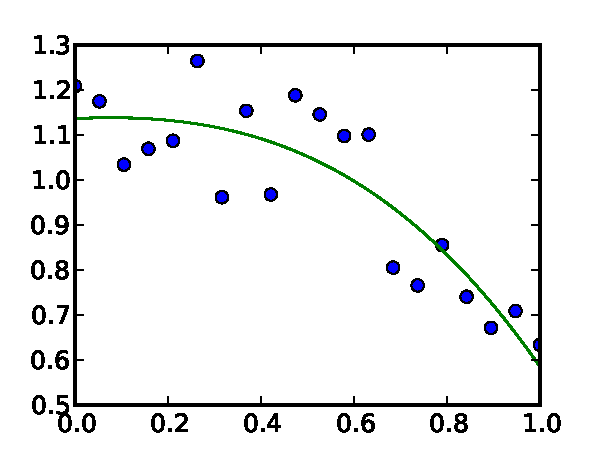
\includegraphics[width=\textwidth]{plwfigis/CursP_2_figure10}

%-------------------------------END CODE
\end{columns}
\end{frame}

%----------------------------FRAME------------------------------------
\begin{frame}[fragile]\frametitle{More Polinomials}
\begin{block}{Chebyshev}
$3x^2+2x-1$
\tiny
\begin{minted} [bgcolor=mybg,frame=lines,bgcolor=mybg,frame=lines,bgcolor=mybg,frame=lines,mathescape]{python}
>>> p = np.polynomial.Polynomial([-1, 2, 3]) # coefs in different order!
>>> p(0)
-1.0
>>> p.roots()
array([-1.        ,  0.33333333])
>>> p.degree()  # In general polynomials do not always expose 'order'
2
\end{minted}

\end{block}

\end{frame}

%----------------------------FRAME 2 cols------------------------------
\begin{frame}[fragile]\frametitle{Example}
\begin{columns}[c]
\column{0.5\textwidth}
\tiny
\begin{minted} [bgcolor=mybg,frame=lines,bgcolor=mybg,frame=lines,bgcolor=mybg,frame=lines,mathescape]{python}
>>> x = np.linspace(-1, 1, 2000)
>>> y = np.cos(x) + 0.3*np.random.rand(2000)
>>> p = np.polynomial.Chebyshev.fit(x, y, 90)
>>> t = np.linspace(-1, 1, 200)
>>> plt.plot(x, y, 'r.')   
[<matplotlib.lines.Line2D object at ...>]
>>> plt.plot(t, p(t), 'k-', lw=3)   
[<matplotlib.lines.Line2D object at ...>]
\end{minted}

\column{0.5\textwidth}
%-------------------------------CODE
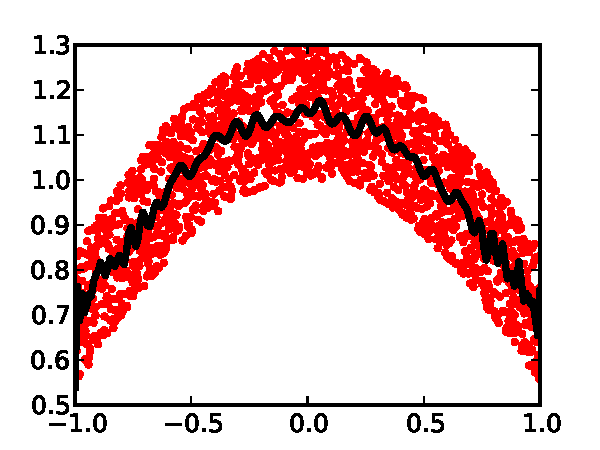
\includegraphics[width=\textwidth]{plwfigis/CursP_2_figure11}

%-------------------------------END CODE
\end{columns}
\end{frame}



\section{Matplotlib}

\subsection{Introduction}
%----------------------------FRAME------------------------------------
\begin{frame}[fragile]\frametitle{Matplotlib Vs Pylab}
\begin{block}{Matplotlib}
\tiny
matplotlib is probably the single most used Python package for 2D-graphics
\end{block}
\begin{block}{Pylab}
\tiny
pylab provides a procedural interface to the matplotlib object-oriented plotting library. It is modeled closely after Matlab(TM). Therefore, the majority of plotting commands in pylab have Matlab(TM) analogs with similar arguments
\end{block}
\begin{block}{Conclusion}
\tiny
Learn Pylab
\end{block}
\begin{block}{How to bring pylab to work}
\tiny
\begin{itemize}
    \item Fom any editor import it
\tiny
\begin{minted} [bgcolor=mybg,frame=lines,bgcolor=mybg,frame=lines,bgcolor=mybg,frame=lines,mathescape]{python}
from pylab import *
\end{minted}
\item start iPython with pylab
\begin{verbatim}
    $ ipython --pylab
\end{verbatim}
\end{itemize}

\end{block}


\end{frame}

%----------------------------FRAME------------------------------------
\begin{frame}[fragile]\frametitle{Process}
\begin{block}{Learn by example}
To show how it works lets make an evolutive graphic
\end{block}

\end{frame}



\subsection{Figures and Subplots}

%----------------------------FRAME 2 cols------------------------------
\begin{frame}[fragile]\frametitle{Simple plot}
\begin{columns}[c]
\column{0.6\textwidth}
\begin{block}{Create data and plot it}
\tiny
\begin{minted} [bgcolor=mybg,frame=lines,bgcolor=mybg,frame=lines,bgcolor=mybg,frame=lines,mathescape]{python}
import pylab as pl
import numpy as np

X = np.linspace(-np.pi, np.pi, 256, endpoint=True)
C, S = np.cos(X), np.sin(X)

pl.plot(X, C)
pl.plot(X, S)

pl.show()
\end{minted}

\end{block}

\column{0.4\textwidth}

%------------------------------CODE
%-------------------------------CODE
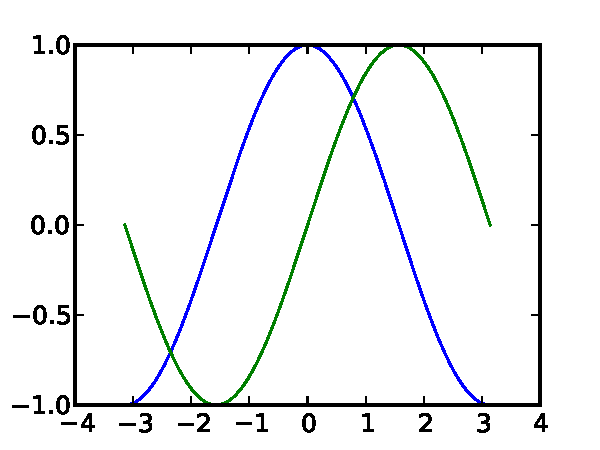
\includegraphics[width=\textwidth]{plwfigis/CursP_2_figure12}

%-------------------------------END CODE
\end{columns}
\end{frame}
%----------------------------FRAME 2 cols------------------------------
\begin{frame}[fragile]\frametitle{Instantiating defaults}
\begin{columns}[c]
\column{0.7\textwidth}
\tiny
\begin{minted} [bgcolor=mybg,frame=lines,bgcolor=mybg,frame=lines,bgcolor=mybg,frame=lines,mathescape]{python}
import pylab as pl
import numpy as np
# Create a figure of size 8x6 points, 80 dots per inch
pl.figure(figsize=(8, 6), dpi=80)
# Create a new subplot from a grid of 1x1
pl.subplot(1, 1, 1)
X = np.linspace(-np.pi, np.pi, 256, endpoint=True)
C, S = np.cos(X), np.sin(X)
# Plot cosine with a blue continuous line of width 1 (pixels)
pl.plot(X, C, color="blue", linewidth=1.0, linestyle="-")
# Plot sine with a green continuous line of width 1 (pixels)
pl.plot(X, S, color="green", linewidth=1.0, linestyle="-")
# Set x limits
pl.xlim(-4.0, 4.0)
# Set x ticks
pl.xticks(np.linspace(-4, 4, 9, endpoint=True))
# Set y limits
pl.ylim(-1.0, 1.0)
# Set y ticks
pl.yticks(np.linspace(-1, 1, 5, endpoint=True))
# Save figure using 72 dots per inch
# savefig("exercice_2", dpi=72)
# Show result on screen
pl.show()
\end{minted}

\column{0.3\textwidth}
%-------------------------------CODE
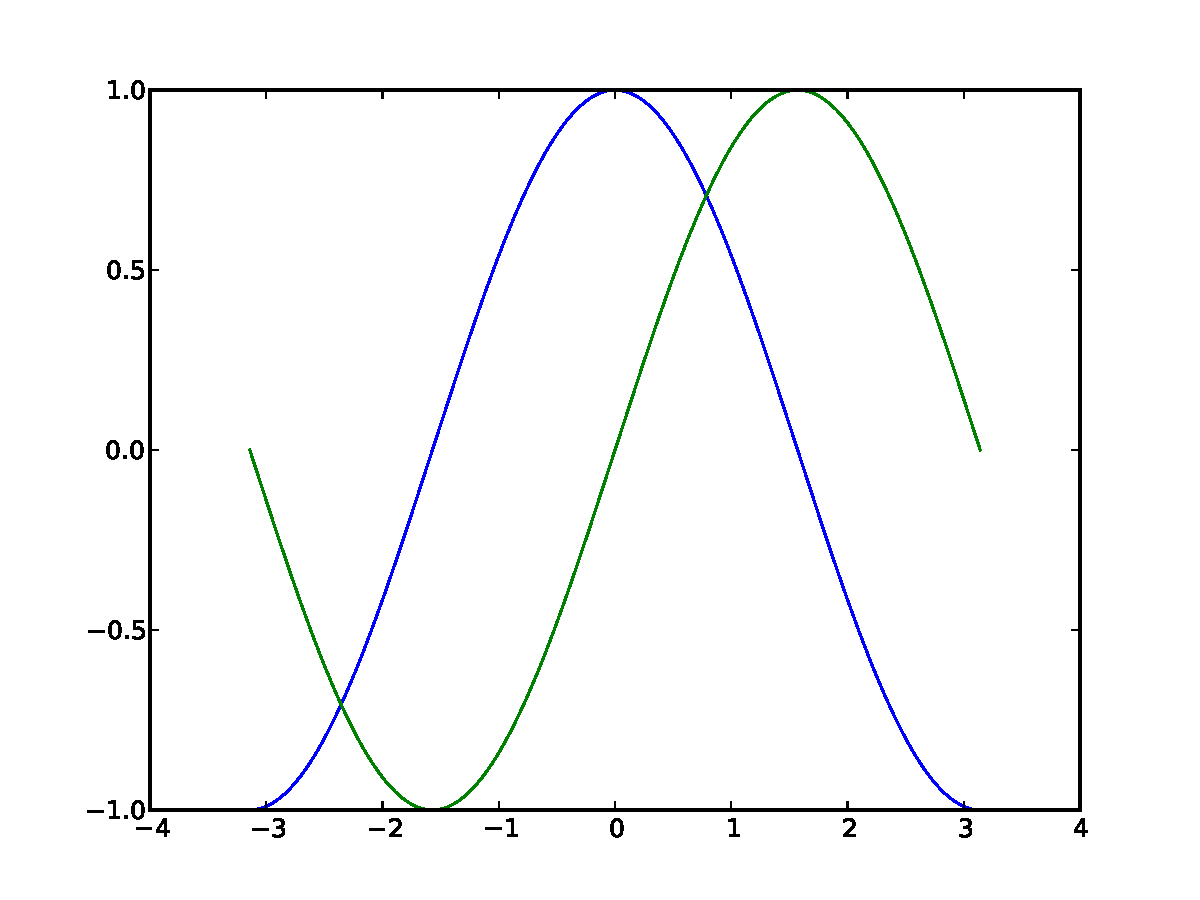
\includegraphics[width=\textwidth]{plwfigis/CursP_2_figure13}

%-------------------------------END CODE
\end{columns}
\end{frame}
%----------------------------FRAME 2 cols------------------------------
\begin{frame}[fragile]\frametitle{Changing colors and line widths}
\begin{columns}[c]
\column{0.6\textwidth}
\begin{block}{First step}
\tiny
the cosine in blue and the sine in red and a slighty thicker line for both of them. We’ll also slightly alter the figure size to make it more horizontal.
\begin{minted} [bgcolor=mybg,frame=lines,bgcolor=mybg,frame=lines,bgcolor=mybg,frame=lines,mathescape]{python}
...
pl.figure(figsize=(10, 6), dpi=80)
pl.plot(X, C, color="blue", linewidth=2.5, linestyle="-")
pl.plot(X, S, color="red",  linewidth=2.5, linestyle="-")
...
\end{minted}

\end{block}

\column{0.4\textwidth}
%-------------------------------CODE
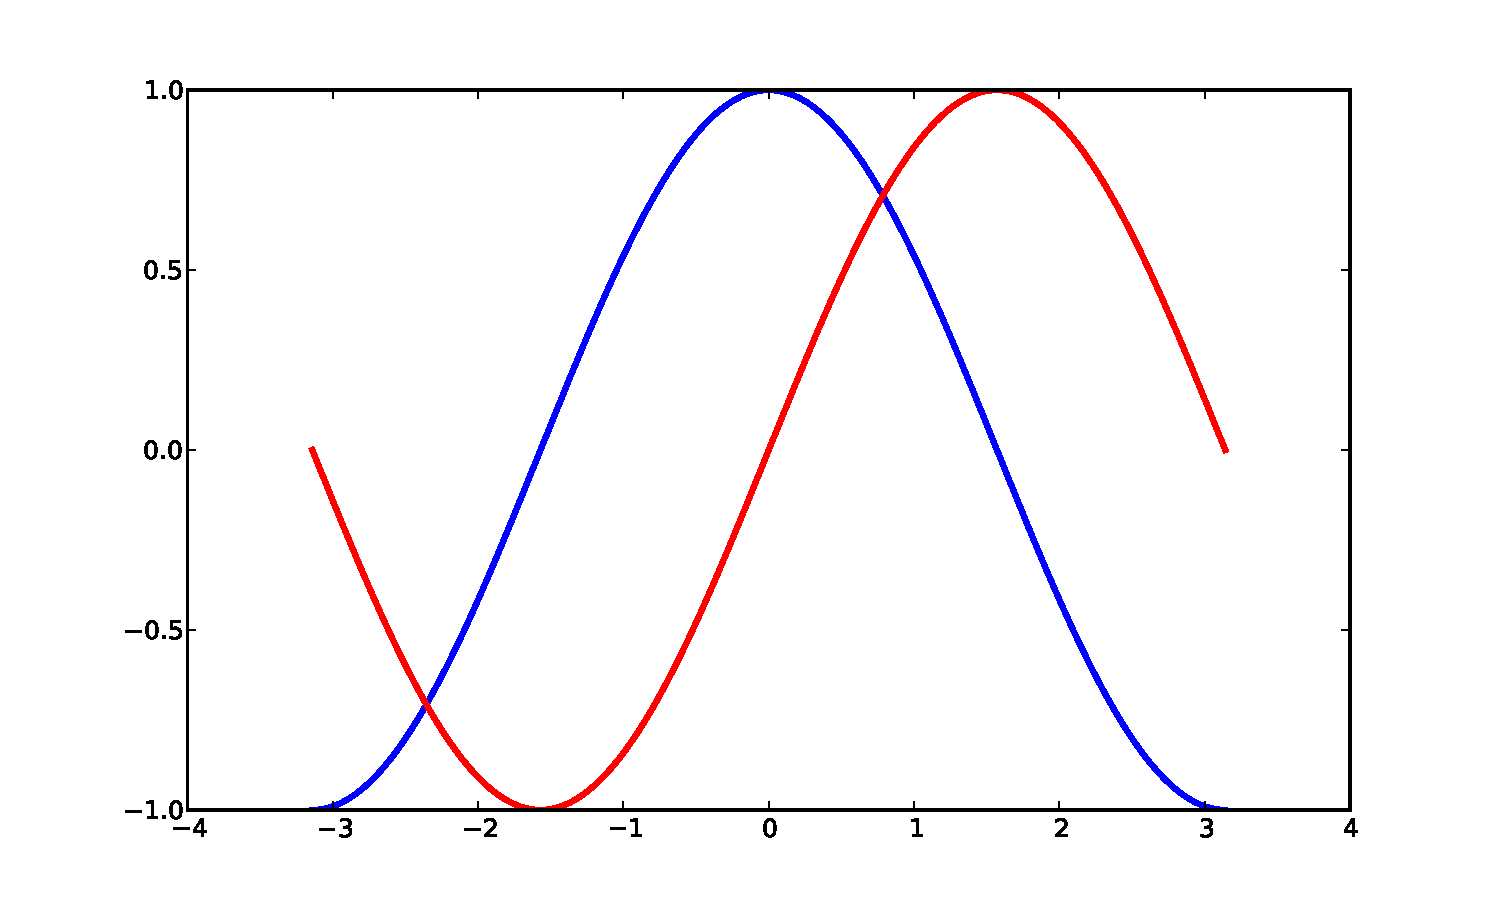
\includegraphics[width=\textwidth]{plwfigis/CursP_2_figure14}

%-------------------------------END CODE
\end{columns}
\end{frame}

%----------------------------FRAME 2 cols------------------------------
\begin{frame}[fragile]\frametitle{Setting limits}
\begin{columns}[c]
\column{0.6\textwidth}
\begin{block}{Second step}
\tiny
Lets adjust a little bit the figure limits
\begin{minted} [bgcolor=mybg,frame=lines,bgcolor=mybg,frame=lines,bgcolor=mybg,frame=lines,mathescape]{python}
...
pl.xlim(X.min() * 1.1, X.max() * 1.1)
pl.ylim(C.min() * 1.1, C.max() * 1.1)
...
\end{minted}

\end{block}

\column{0.4\textwidth}
%-------------------------------CODE
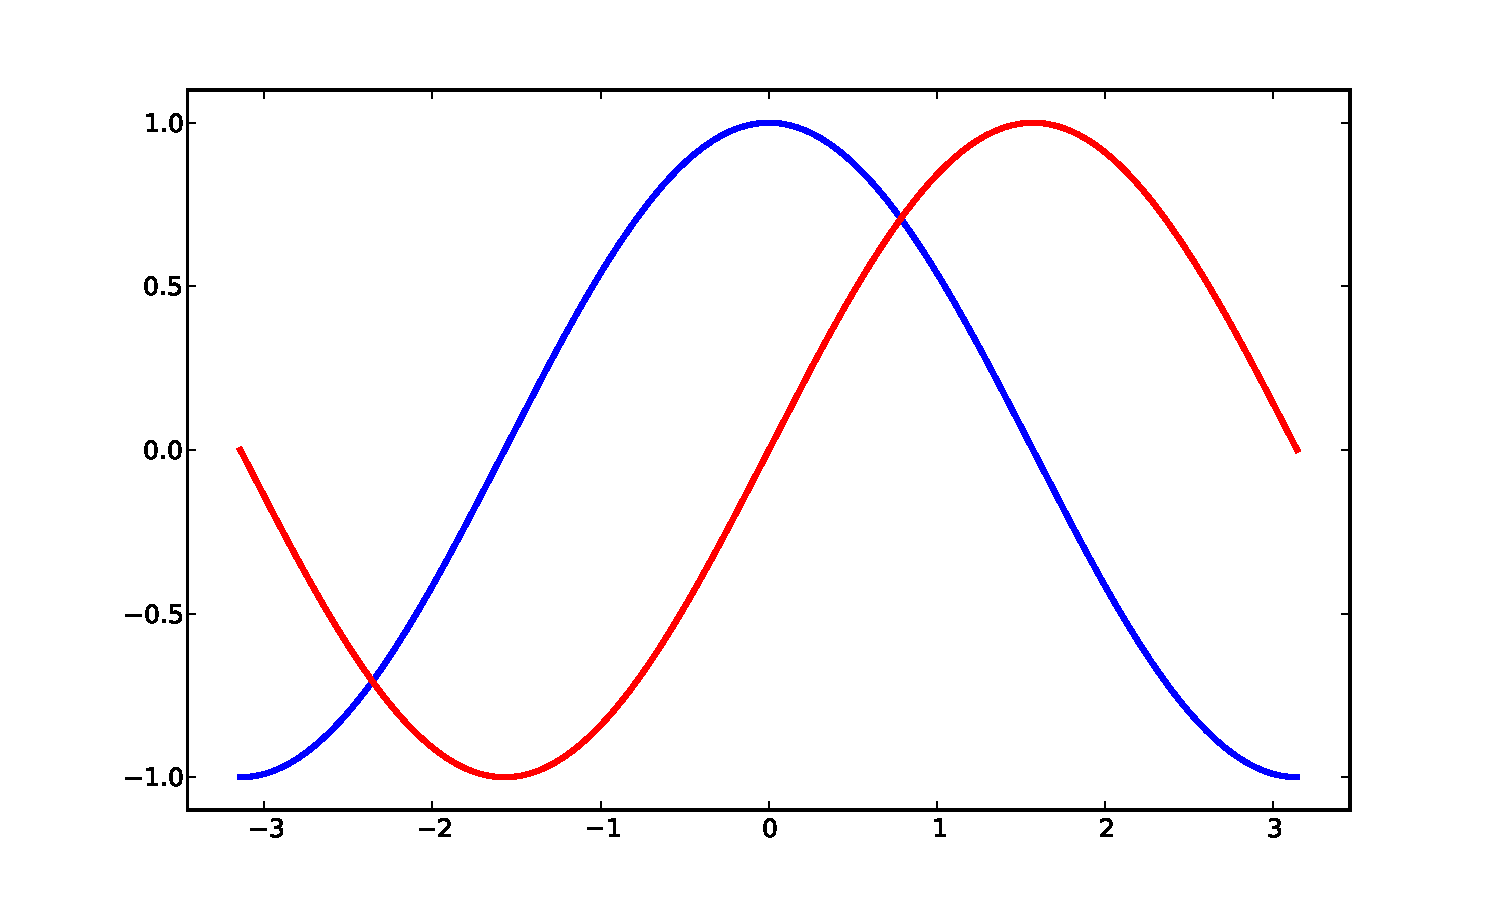
\includegraphics[width=\textwidth]{plwfigis/CursP_2_figure15}

%-------------------------------END CODE
\end{columns}
\end{frame}


%----------------------------FRAME 2 cols------------------------------
\begin{frame}[fragile]\frametitle{Setting tickss}
\begin{columns}[c]
\column{0.6\textwidth}
\begin{block}{Third step}
\tiny
Change figure tiks
\begin{minted} [bgcolor=mybg,frame=lines,bgcolor=mybg,frame=lines,bgcolor=mybg,frame=lines,mathescape]{python}
...
pl.xticks([-np.pi, -np.pi/2, 0, np.pi/2, np.pi])
pl.yticks([-1, 0, +1])
...
\end{minted}

\end{block}

\column{0.4\textwidth}
%-------------------------------CODE
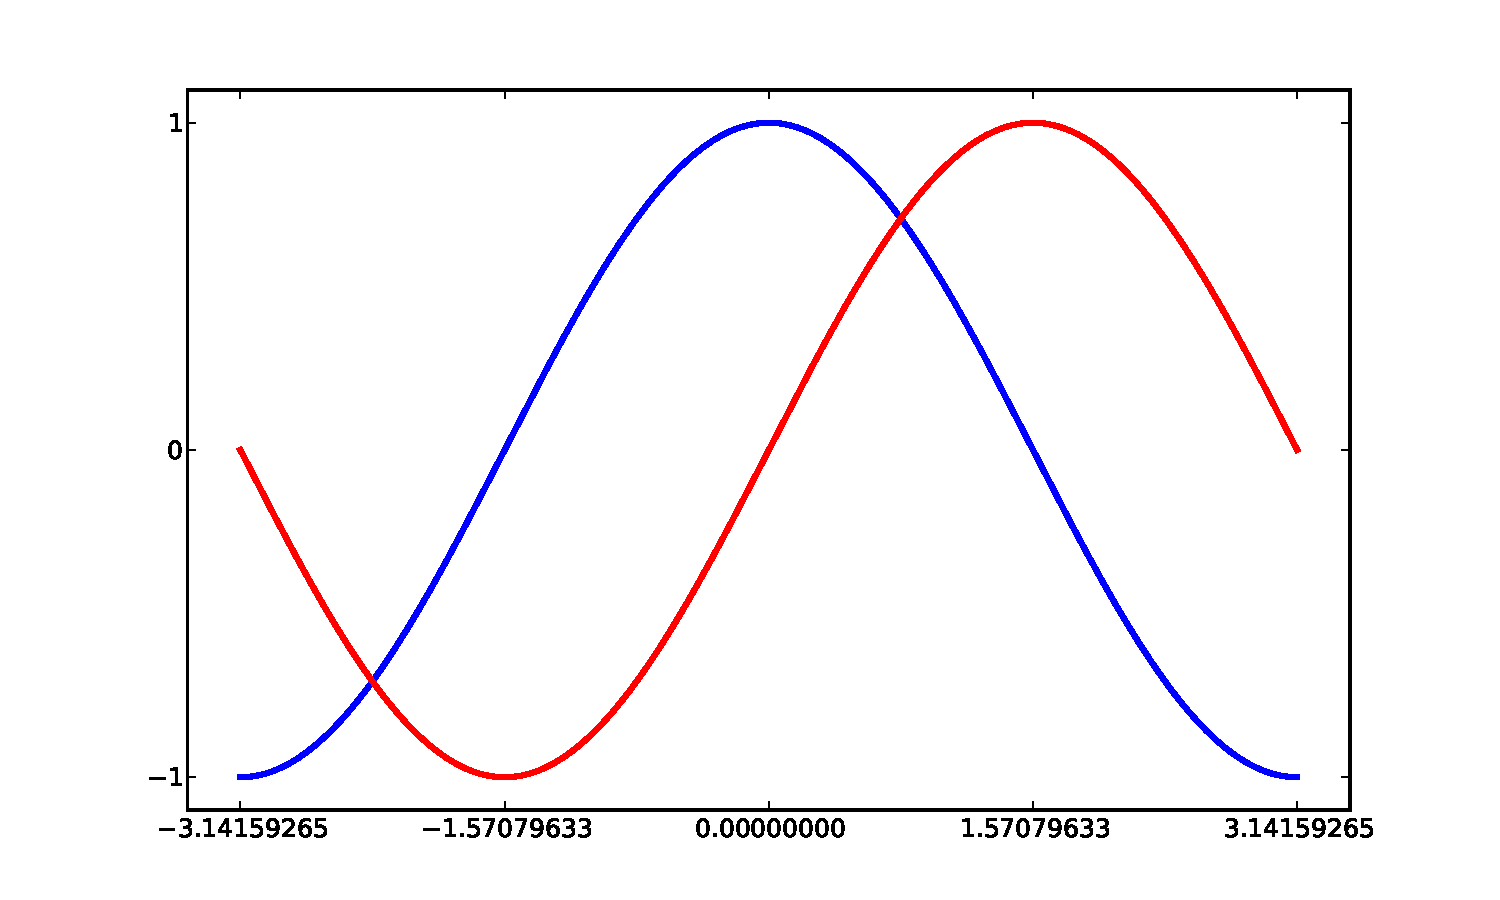
\includegraphics[width=\textwidth]{plwfigis/CursP_2_figure16}

%-------------------------------END CODE
\end{columns}
\end{frame}


%----------------------------FRAME 2 cols------------------------------
\begin{frame}[fragile]\frametitle{Setting tick labels}
\begin{columns}[c]
\column{0.6\textwidth}
\begin{block}{Forth step}
\tiny
Change figure tiks' labels
\begin{minted} [bgcolor=mybg,frame=lines,bgcolor=mybg,frame=lines,bgcolor=mybg,frame=lines,mathescape]{python}
...
pl.xticks([-np.pi, -np.pi/2, 0, np.pi/2, np.pi],
[r'$-\pi$', r'$-\pi/2$', r'$0$', r'$+\pi/2$', r'$+\pi$'])

pl.yticks([-1, 0, +1],
          [r'$-1$', r'$0$', r'$+1$'])
...
\end{minted}

\end{block}

\column{0.4\textwidth}
%-------------------------------CODE
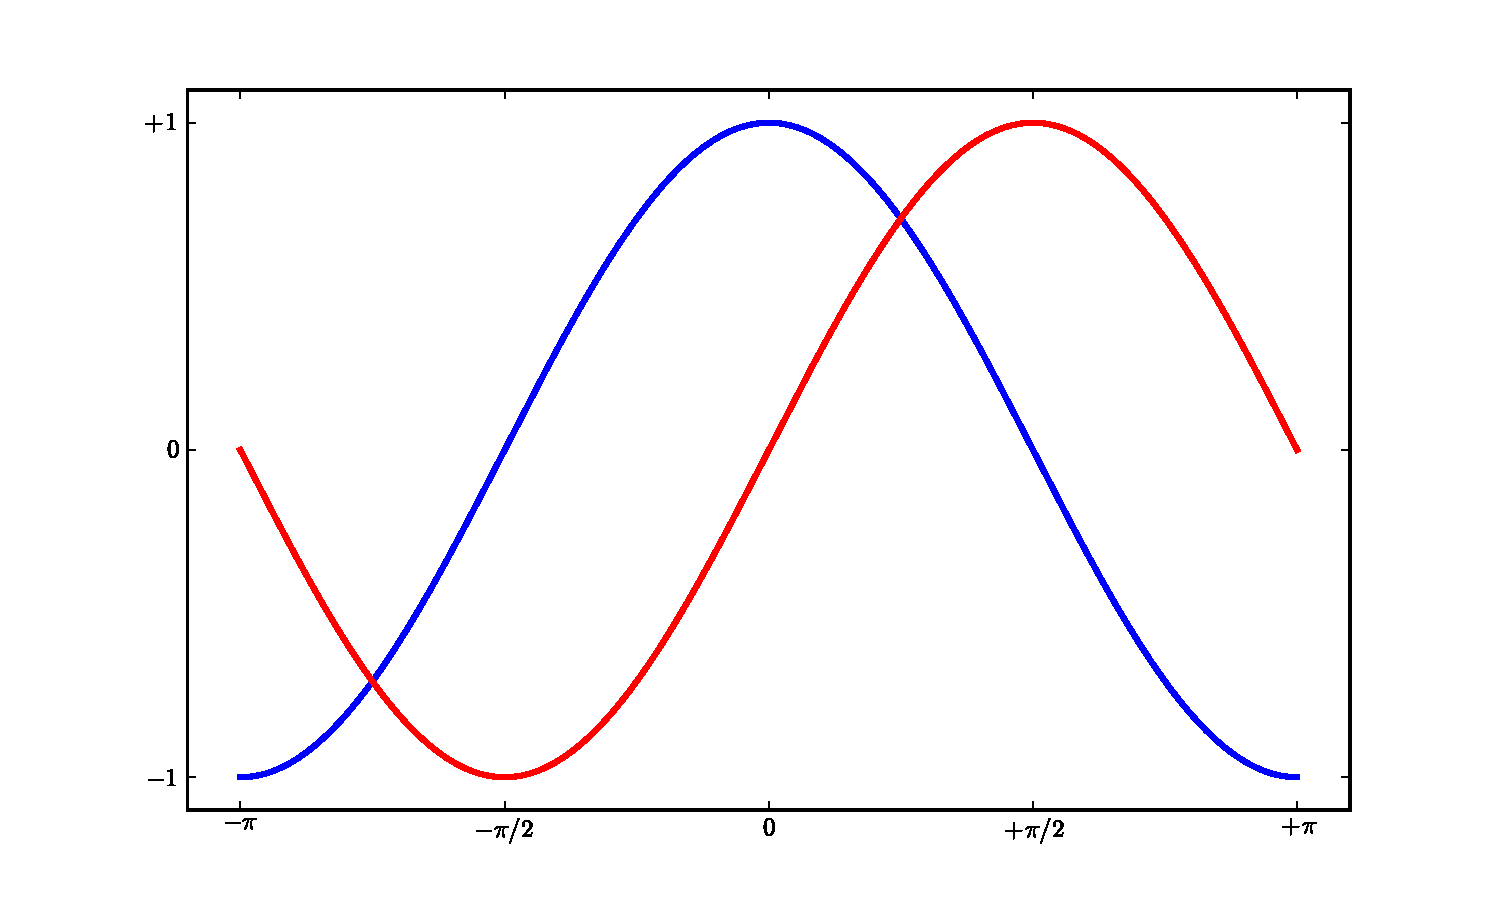
\includegraphics[width=\textwidth]{plwfigis/CursP_2_figure17}

%-------------------------------END CODE
\end{columns}
\end{frame}



%----------------------------FRAME 2 cols------------------------------
\begin{frame}[fragile]\frametitle{Moving spines}
\begin{columns}[c]
\column{0.6\textwidth}
\begin{block}{Forth step}
\tiny
Change axis positions
\begin{minted} [bgcolor=mybg,frame=lines,bgcolor=mybg,frame=lines,bgcolor=mybg,frame=lines,mathescape]{python}
...
ax = pl.gca()  # gca stands for 'get current axis'
ax.spines['right'].set_color('none')
ax.spines['top'].set_color('none')
ax.xaxis.set_ticks_position('bottom')
ax.spines['bottom'].set_position(('data',0))
ax.yaxis.set_ticks_position('left')
ax.spines['left'].set_position(('data',0))
...
\end{minted}

\end{block}

\column{0.4\textwidth}
%-------------------------------CODE
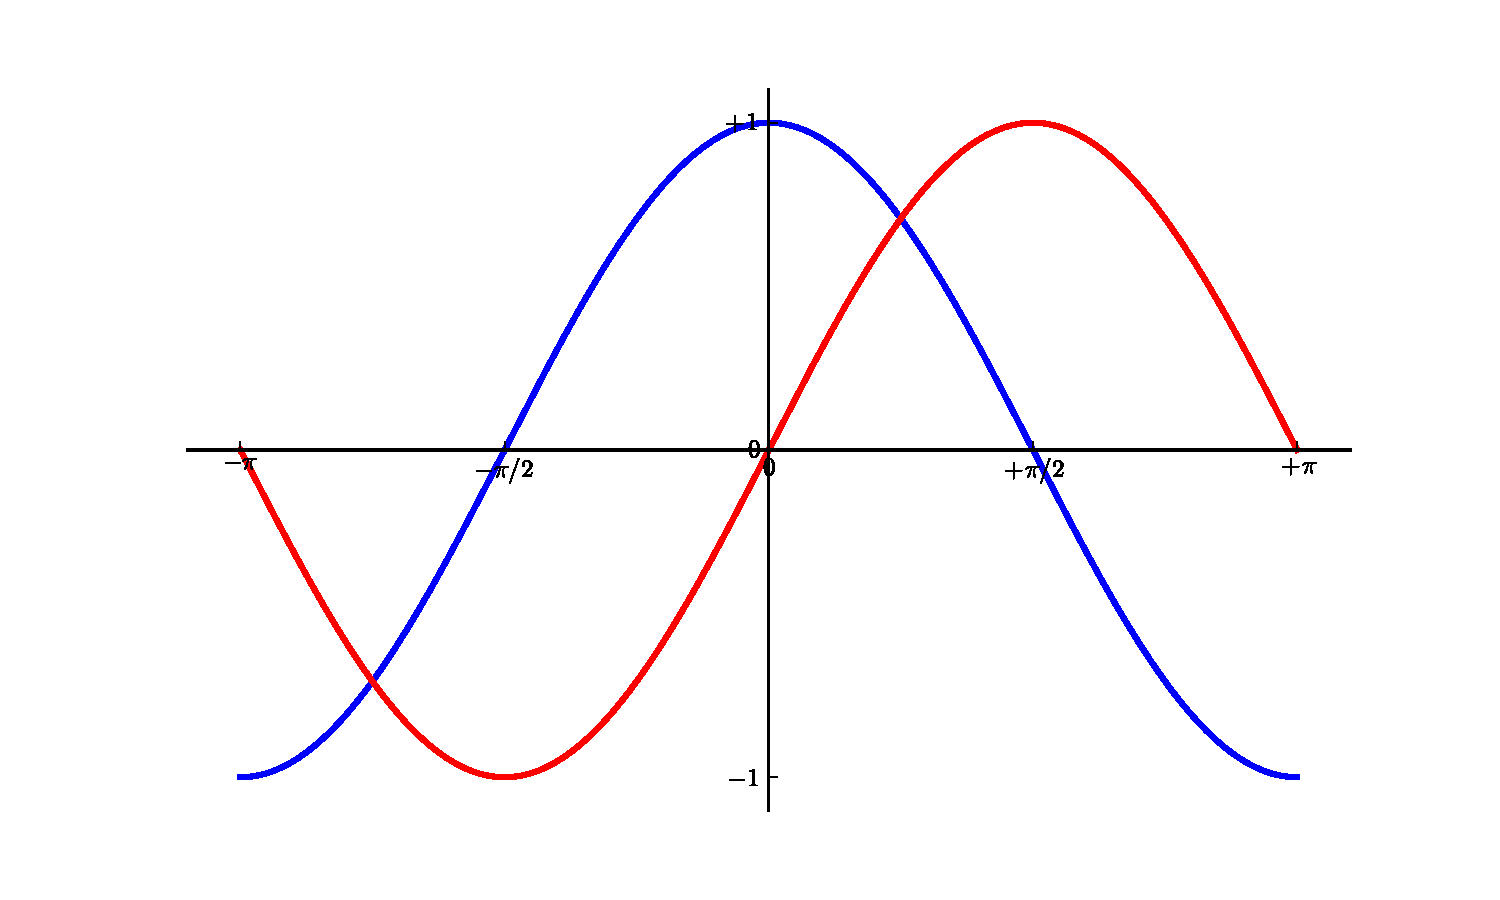
\includegraphics[width=\textwidth]{plwfigis/CursP_2_figure18}

%-------------------------------END CODE
\end{columns}
\end{frame}




%----------------------------FRAME 2 cols------------------------------
\begin{frame}[fragile]\frametitle{Adding a legend}
\begin{columns}[c]
\column{0.6\textwidth}
\begin{block}{Going on...}
\tiny
\begin{minted} [bgcolor=mybg,frame=lines,bgcolor=mybg,frame=lines,bgcolor=mybg,frame=lines,mathescape]{python}
...
pl.plot(X, C, color="blue", linewidth=2.5, linestyle="-",
        label="cosine")
pl.plot(X, S, color="red",  linewidth=2.5, linestyle="-",
        label="sine")

pl.legend(loc='upper left')
...
\end{minted}

\end{block}

\column{0.4\textwidth}
%-------------------------------CODE
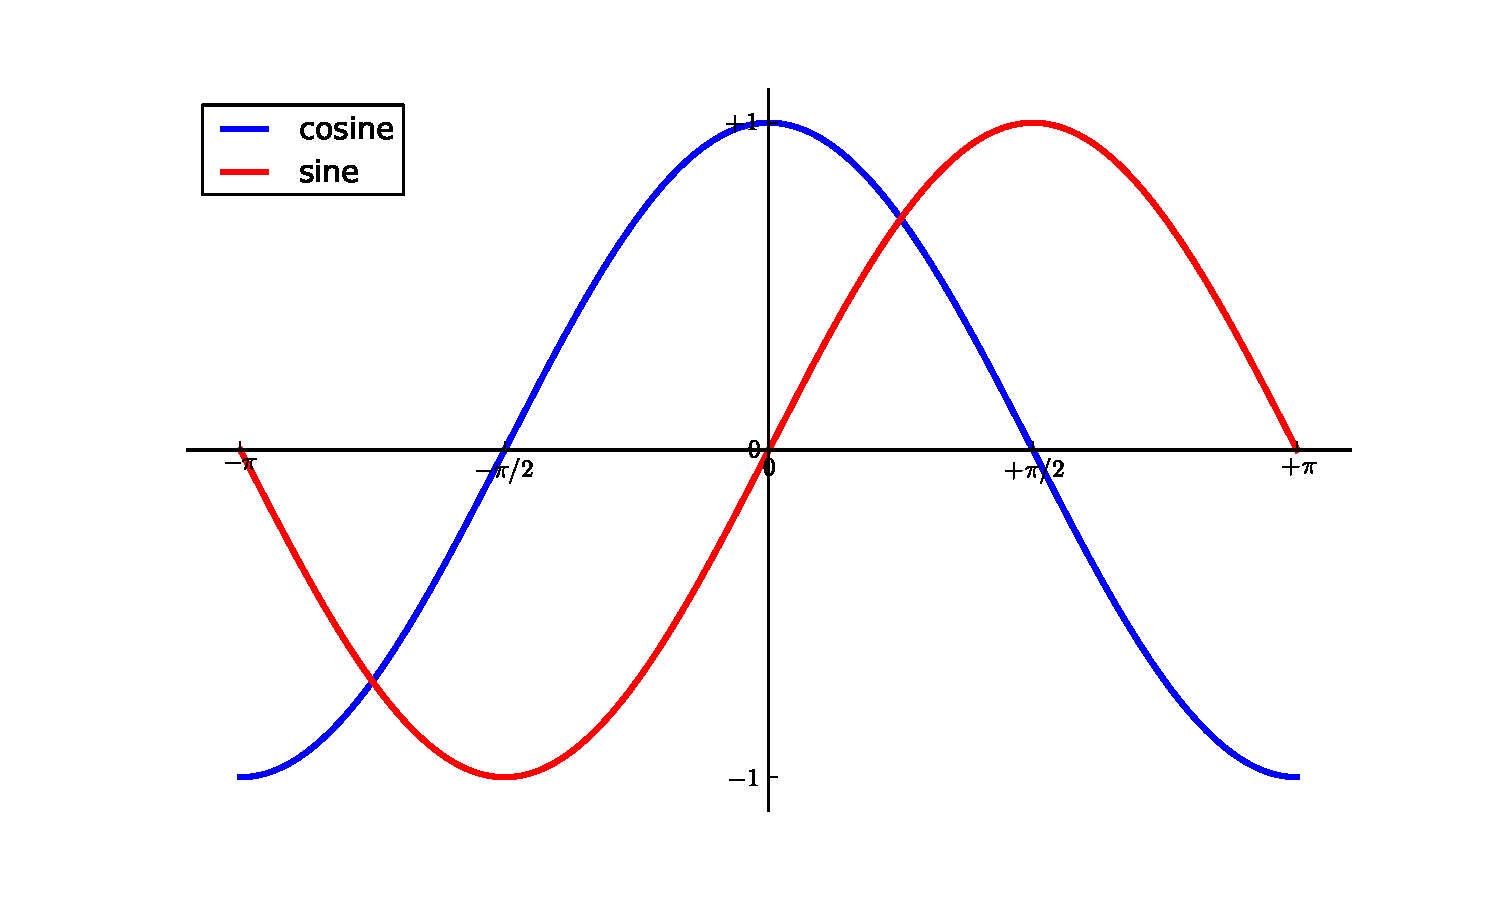
\includegraphics[width=\textwidth]{plwfigis/CursP_2_figure19}

%-------------------------------END CODE
\end{columns}
\end{frame}






%----------------------------FRAME 2 cols------------------------------
\begin{frame}[fragile]\frametitle{Annotate some points}
\begin{columns}[c]
\column{0.7\textwidth}
\begin{block}{Going on...}
\tiny
\begin{minted} [bgcolor=mybg,frame=lines,bgcolor=mybg,frame=lines,bgcolor=mybg,frame=lines,mathescape]{python}
...
t = 2 * np.pi / 3
pl.plot([t, t], [0, np.cos(t)], color='blue', linewidth=2.5,
         linestyle="--")
pl.scatter([t, ], [np.cos(t), ], 50, color='blue')

pl.annotate(r'$sin(\frac{2\pi}{3})=\frac{\sqrt{3}}{2}$',
            xy=(t, np.sin(t)), xycoords='data',
            xytext=(+10, +30), textcoords='offset points', 
            fontsize=16,arrowprops=dict(arrowstyle="->", 
            connectionstyle="arc3,rad=.2"))

pl.plot([t, t],[0, np.sin(t)], color='red', linewidth=2.5,
            linestyle="--")
pl.scatter([t, ],[np.sin(t), ], 50, color='red')

pl.annotate(r'$cos(\frac{2\pi}{3})=-\frac{1}{2}$',
            xy=(t, np.cos(t)), xycoords='data',
            xytext=(-90, -50), textcoords='offset points',
            fontsize=16,arrowprops=dict(arrowstyle="->", 
            connectionstyle="arc3,rad=.2"))
...
\end{minted}

\end{block}

\column{0.4\textwidth}
%-------------------------------CODE
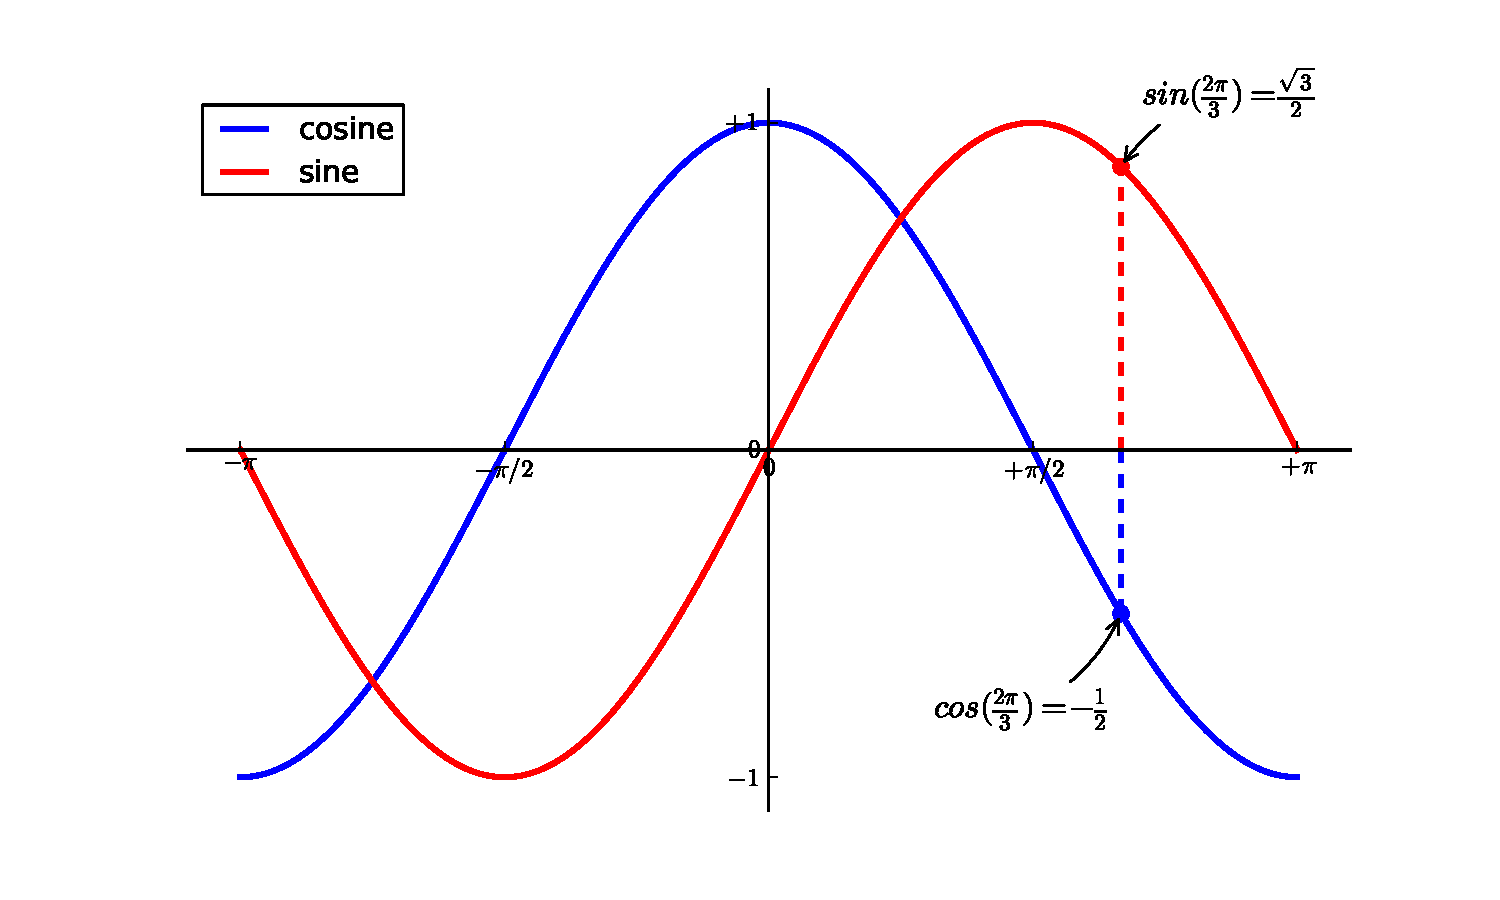
\includegraphics[width=\textwidth]{plwfigis/CursP_2_figure20}

%-------------------------------END CODE
\end{columns}
\end{frame}







%----------------------------FRAME 2 cols------------------------------
\begin{frame}[fragile]\frametitle{Finally...}
\begin{columns}[c]
\column{0.7\textwidth}
\begin{block}{The last detail}
\tiny
\begin{minted} [bgcolor=mybg,frame=lines,bgcolor=mybg,frame=lines,bgcolor=mybg,frame=lines,mathescape]{python}
...
for label in ax.get_xticklabels() + ax.get_yticklabels():
    label.set_fontsize(16)
    label.set_bbox(dict(facecolor='white', edgecolor='None', 
    alpha=0.65))
...
\end{minted}

\end{block}

\column{0.4\textwidth}
%-------------------------------CODE
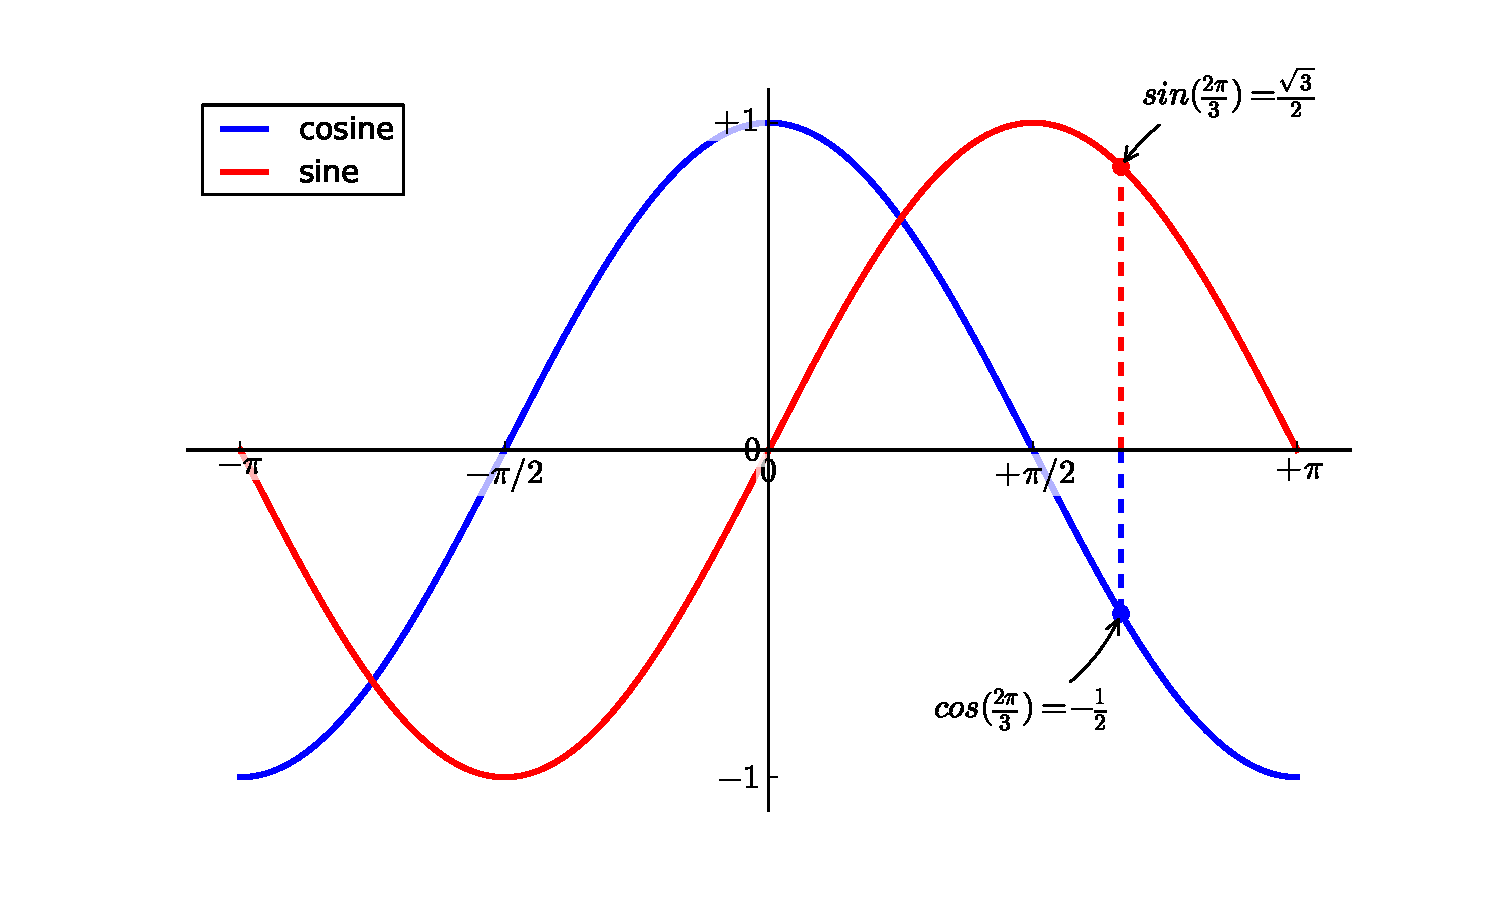
\includegraphics[width=\textwidth]{plwfigis/CursP_2_figure21}

%-------------------------------END CODE
\end{columns}
\end{frame}





\subsection{Axes and further control of figures}

%----------------------------FRAME------------------------------------
\begin{frame}[fragile]\frametitle{Creating figures}
\begin{block}{Parameters}
\begin{description}
    \item[num] number of figure, start by 1!!!
\item [figsize]	figure.figsize,figure size in in inches (width, height)
\item [dpi] figure.dpi ,resolution in dots per inch
\item [facecolor] figure.facecolor, color of the drawing background
\item [edgecolor] figure.edgecolor, color of edge around the drawing background
\item [frameon] True, draw figure frame or not 
\end{description}
\end{block}

\end{frame}


%----------------------------FRAME 2 cols------------------------------
\begin{frame}[fragile]\frametitle{Subplots}
\begin{columns}[c]
\column{0.5\textwidth}
\tiny
\begin{minted} [bgcolor=mybg,frame=lines,bgcolor=mybg,frame=lines,bgcolor=mybg,frame=lines,mathescape]{python}
pl.figure(figsize=(6, 4))
pl.subplot(2, 2, 1)
pl.xticks(())
pl.yticks(())
pl.text(0.5, 0.5, 'subplot(2,2,1)', ha='center',
     va='center',size=20, alpha=.5)

pl.subplot(2, 2, 2)
pl.xticks(())
pl.yticks(())
pl.text(0.5, 0.5, 'subplot(2,2,2)', ha='center', 
     va='center', size=20, alpha=.5)

pl.subplot(2, 2, 3)
pl.xticks(())
pl.yticks(())

pl.text(0.5, 0.5, 'subplot(2,2,3)', ha='center', 
    va='center', size=20, alpha=.5)

pl.subplot(2, 2, 4)
pl.xticks(())
pl.yticks(())
pl.text(0.5, 0.5, 'subplot(2,2,4)', ha='center', 
        va='center', size=20, alpha=.5)

pl.tight_layout()
pl.show()
\end{minted}

\column{0.5\textwidth}
%-------------------------------CODE
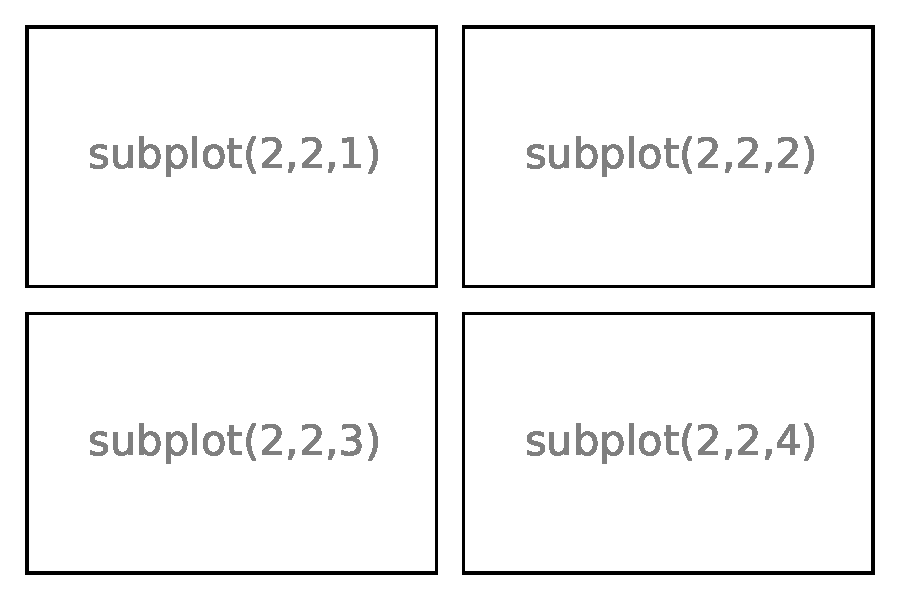
\includegraphics[width=\textwidth]{plwfigis/CursP_2_figure22}

%-------------------------------END CODE
\end{columns}
\end{frame}


%-------------------------------------------------------------------
%---------------------------FINAL FRAME-----------------------------
%-------------------------------------------------------------------



\begin{frame}[Thank you!] 
  \begin{center}
    \centering 
\includegraphics[width=0.5\linewidth]{figs/question_mark}
  \end{center}
\end{frame}


\end{document}
